\documentclass{MScthesisITEM}

% this package is just to generate text for demo-purposes
\usepackage{blindtext}
\usepackage{todonotes}
\usepackage[pdf,tmpdir]{graphviz}


\title{NUTS Uplink Authentication} % The title of your assignement; NB use \newlinetitle to start a newline
\author{Tarjei Husøy} % Your firstname and lastname
\professor{Stig Frode Mjølsnes, ITEM} % Affiliation = ITEM for instance
\supervisor{Roger Birkeland, IET}

%% Uncomment the following in case you want subfigures; note that there will be a warning for the caption package
\let\subcaption\undefined
\let\subfloat\undefined
\usepackage[width=.85\textwidth]{caption}
\usepackage{subcaption}

\DeclareGraphicsExtensions{.pdf,.png,.jpg}
\graphicspath{{./figs/}}

\loadglsentries{glossary}
\makeglossaries

\setlength\epigraphwidth{12cm}
\setlength\epigraphrule{0pt}

\lstset{
    showspaces=false,
    showstringspaces=false,
    showtabs=false,
    basicstyle=\footnotesize,
    numberstyle=\footnotesize,
    tabsize=2,
    otherkeywords={with, as},
    language=Python,
    breaklines=true,
    captionpos=t,
}

\begin{document}
%\listoftodos
%\clearpage
\selectlanguage{english}
\pagenumbering{roman}
\pagestyle{plain}

%% Only for the project; comment out the line below for the master's thesis; the front page will be generated automatically by DAIM
\titleITEM

%% Only for the master's thesis; for the project report the description is taken from It's Learning and added by the department
% \selectlanguage{english} % Change to 'norsk' if you are writing in Norwegian
%\begin{titlingpage}

\noindent
\begin{tabular}{@{}p{4cm}l}
\textbf{Title:} 	& \thetitle \\
\textbf{Student:}	& \theauthor \\
\end{tabular}

\vspace{4ex}
\noindent\textbf{Problem description:}
\vspace{2ex}

A new shared-key HMAC authentication protocol for the uplink from the ground station to the NUTS CubeSat has been proposed [1].

This assignment will continue the development of this authenticated protocol design by focusing on the problem of key management, including generation, distribution, and renewal of cryptographic keys.  A very important part of this problem is how to manage a hard reset of the satellite runtime system and be able to re-establish the cryptographic association in a secure way.

The proposed solution should be supported by an experimental implementation that validates that expected failure modes can be handled. If time allows, the student should consider using
electronic circuitry for key generation which can be randomized by available space radiation.

[1]  M. Munch.  Integration and verification of a keyed-message authentication scheme based on broadcast timestamps for NUTS. Master's thesis, NTNU, Trondheim, July 2014.

\vspace{6ex}

\noindent
\begin{tabular}{@{}p{4cm}l}
\textbf{Responsible professor:} 	& \theprofessor \\
\textbf{Supervisor:}			& \thesupervisor \\
\end{tabular}

\end{titlingpage}

% \cleardoublepage

%% There must be an abstract in English, even though the main text is in Norwegian
\selectlanguage{english}
\pagestyle{empty}
\begin{abstract}

This project demonstrates \gls{nap}, a new two-way authenticated communications protocol suitable for open networks, such as open Wi-Fi networks or ham radio links, originally intended for usage in the \gls{nuts} CubeSat project. Due to legal restrictions on ham radio links about encoding data, the protocol is intended for applications which need authentication and source integrity, but not confidentiality.

The protocol is based on pre-shared keys and \glspl{mac}, and establishes sessions with sequence numbers to defeat replay attacks. The protocol contains a feature to re-negotiate long-term keys in case they're compromised.

The protocol is verified through scyther, a utility to verify formal security properties of protocols. Potential risks, implementation details and failure modes are discussed, and a sample implementation can be found at \url{https://github.com/thusoy/nuts-auth}. Example usage of the implementation for both the client and server is provided in this paper.

\end{abstract}

\cleardoublepage

%% Only for the master's thesis; if the main text is in English and you can write Norwegian, there must be an abstract in Norwegian as well.
% \selectlanguage{norsk}
% \include{abstract_norwegian}
% \cleardoublepage

\selectlanguage{english}% Change to 'norsk' if you are writing in Norwegian

\renewcommand{\abstractname}{Acknowledgements}
\begin{abstract}

I want to thank my supervising professor at \gls{item}, Stig Frode Mjølsnes, who has been very helpful throughout the project, providing lots of valuable feedback and healthy discussions on both this subject and everything else we've found interesting this semester. Other people on the staff at ITEM and \gls{iet} have also been very forthcoming in providing me with lots of hardware to play around with, for which I'm very grateful.

My appreciation for Roger Birkeland and Amund Gjersvik, both from IET, also needs to mentioned, as without their work on getting the NUTS project on its feet this project would never have existed.

I'd also like to extend my gratitude to Martin Kirkholt Melhus, who proofread and came with valuable feedback on an early version of this report.

\end{abstract}

\cleardoublepage

% similarly you may add a separate acknowledgments page

\tableofcontents*
\cleardoublepage

%% include if relevant
\listoffigures
\cleardoublepage

%% include if relevant
\listoftables
\cleardoublepage

%% include if relevant
% \listofalgorithms
% \addcontentsline{toc}{chapter}{List of Algorithms}
% \cleardoublepage

%% include if relevant
\printglossary[title=List of Symbols, style=long]
\cleardoublepage
\glsaddall[]

%% include if relevant
\printglossary[title=List of Acronyms,type=\acronymtype] % prints just the list of acronyms
\cleardoublepage

\pagenumbering{arabic}
\pagestyle{ruled}
\chapter{Introduction}
\label{chp:introduction}

\section{The Problem Description}\label{sec:problem_description}

The original problem description states that the project should be aimed at key management based upon the previous protocol developed for the NUTS project. However, we found major flaws in the underlying protocol, which prevented any further work based on that protocol. We thus focused this project on re-designing the protocol to make sure that NUTS has a trusted transport layer protocol they can build upon. We also shifted the focus away from the NUTS hardware towards a general purpose implementation that would work on all platforms, targeting a setup based on Raspberry Pis communicating over open, unencrypted Wi-Fi. This enables the setup to also be re-used for another course at NTNU, TTM4137 Wireless Network Security, enabling more students to analyze the protocol and try to break it.

The goal of this project is thus to fully describe a new, mutually authenticated protocol, analyze it's security properties, and verify that it works through a sample implementation running on Raspberry Pis.

\section{Results}\label{sec:results}

\begin{figure}[ht!]
\centering
    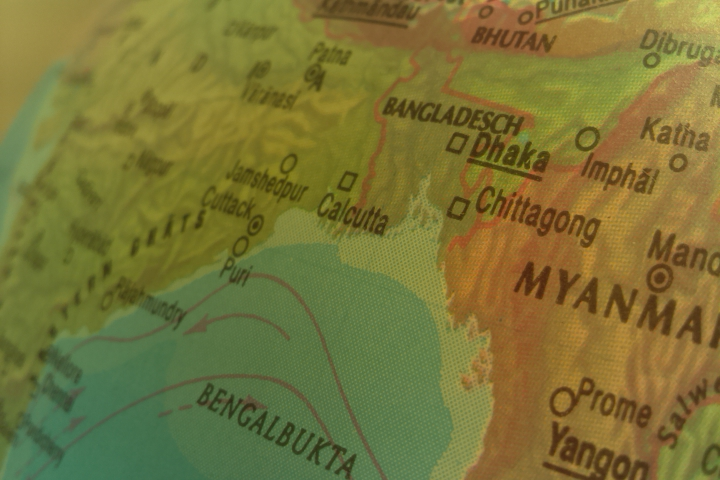
\includegraphics[width=110mm]{orbit-bengal}
    \caption{Image of the Bay of Bengal as taken from the "satellite" in our test environment.}\label{fig:orbit-bengal}
\end{figure}

Two example use cases were developed; one simple "Hello, world" application, and one that could fetch and re-assemble fragmented images from the server. Both of the use cases were tested on the Raspberry Pis in the test environment and completed successfully, using the sample implementation given. The result of the latter, an image from the "satellite" orbiting a globe, can be seen in \autoref{fig:orbit-bengal}. The test environment is documented further in \autoref{chp:experiments}.


\section{Structure of this report}\label{sec:structure}

Before embarking on a description of the protocol, this report will first describe the background for the project and why the protocol is needed, establishing the environment it's intended to operate in. When that's settled, we'll dive into the actual specification of the protocol in \autoref{chp:protocol-description}, taking a step-by-step trip through all the messages exchanged between the parties of a session.

That should bring us to a state where the protocol is well understood. We'll then verify that it adheres to the security properties we intended it to have using a tool called scyther, that's based on formal verification. We'll also briefly discuss how the protocol can be extended and adapted to similar environments.

This brings us into a discussion about random numbers in \autoref{chp:random-numbers}, which is an important prerequisite for the protocol to stay secure. Which again is a natural introduction to failure modes, which we'll discuss in \autoref{chp:failure-modes}. Here we'll look at how the protocol can break, what's necessary to compromise it's integrity, and how it can be mitigated.

That establishes all the theory needed to reason about the protocol, which brings us to the experimental work and the sample implementation. \autoref{chp:experiments} will introduce the API of the sample implementation, and some of the motivation for the choices made. Here we also introduce the test setup and how the protocol have been tested on real hardware.

We then round off in \autoref{chp:conclusions} with some final remarks, and some potential pointers for future work on the protocol.


\section{Terminology}\label{sec:terminology}

Note that \emph{ground station} is used interchangeably with \emph{client} in the rest of this document, and that \emph{satellite} is used interchangeably with \emph{server}. This stems from the project's split focus on both space environments and the test setup. \emph{Packet} and \emph{message} is used somewhat interchangeably for the data unit that is passed between the communicating parties. The symbol $\|$ is used to denote concatenation. MAC-Keccak is a MAC based on Keccak.

\chapter{Background}
\label{chp:background}

\section{NUTS}\label{sec:nuts}

\acrfull{nuts} is a collaborative, cross-domain project at NTNU aimed at launching and operating a CubeSat. A CubeSat is a standardized \(10 cm * 10 cm\) format for satellites that make them fit into launch containers, making the deployment of the satellite easy, cheap and efficient. The NUTS CubeSat is a double CubeSat, meaning it has dimensions of \(20 cm * 10 cm\), quite much smaller than most commercial satellites, but the low cost and relative low impact if anything goes wrong make them ideal subjects for experimenting with space technology.

The NUTS satellite is being designed entirely in-house at NTNU. All components are being designed and made from scratch, based on experience gathered by other CubeSat missions performed by other institutions. CubeSats have been popular among universities, giving students a low-risk arena for playing with high tech. Much of our design is influenced by talks given at CubeSat conferences, papers published and standards written. Notable standards include the \gls{csp} \cite{csp}, a network-layer protocol developed by Aalborg University for their CubeSat missions, and being maintained by their spin-off company Gomspace.

In 2011 Visockas \cite{visockas} conducted a study on the existing practice of securing CubeSat uplinks, and found that none of the satellites reviewed offered any means of authentication. This implies that there's a bunch of satellites orbiting earth open for anyone with a directional antenna and the patience to figure out how the communications protocol works, if it's not already published. NTNU wants to enhance the state of the art in this field with NUTS, by providing strong authentication of the uplink through an easy-to-use interface for implementers.

\gls{csp} offers some functionality similar to TCP/IP in the Internet, offering addressing, checksumming, and an implementation of \gls{udp} and \gls{rdp}. CSP also offers HMAC protection of packets, but does not handle replay attack protection, recommending that this be handled on a different layer by implementers. Thus, for the HMAC feature of CSP to be useful, the application layer protocol has to adhere to some spec as well, effectively adding bloating the authentication over several layers. This makes the authentication layer hard to test, hard to implement correctly and hard to prove secure, and that's why we're not utilizing the HMAC features of CSP and instead wrote our own protocol to handle these issues.

While evaluating the HMAC feature of CSP we performed a light review of the \texttt{libcsp} code, and it seems to us that there's no way to force a CSP server to perform the HMAC check, it's only done if the correct header bit is set on an incoming packet. Thus the feature is practically useless, as an adversary will just not set the HMAC flag and the packets will thus be successfully delivered by the CSP layer. Even if implementers forced this check, we also found that neither HMAC nor the CRC32 checks protected the protocol headers, thus allowing an attacker to re-write addresses and ports for both source and destination without affecting the MAC computation. This needs to be addressed in the CSP standard, as fixing this in one given implementation would render it incompatible with other implementations. GomSpace has been made aware of this issue\footnote{The issue can be tracked here: \url{https://github.com/GomSpace/libcsp/issues/45}}.

CSP also truncates the MAC to a fixed 4 byte size, which might be appropriate for space links, but this small, fixed size makes the protocol very targeted for a given environment, and not particularly flexible. Exactly how NUTS is going to utilize CSP and how it'll be work with \gls{nap} is undefined as of now, but putting \gls{nap} on top of the UDP/RDP offerings by CSP in the different subsystems is one option that allows each system to determine it's need for reliable communication.


\section{Security Model}

The security model used to design the protocol is similar to what's usually assumed on the Internet -- the presence of an active attacker who can read, re-order, modify, delete and remember all messages sent. We assume that the endpoints have not been compromised and do not try to protect against that case, as it's generally infeasible.

Notable is that we're assuming that neither the client nor the satellite is trusted. As the NUTS project bases their communication on ham radio, it's not easily determined where a signal originates. Granted, your antenna is directional and pointed towards the satellite, but this assumes you're trusting every component from the antenna to the ground station computer not to be tampered with, and that there's no other satellites talking the same protocol within your focal area. Ensuring a mutual end-to-end identity verification is where we go a step further than previous work in this area.


\section{Ham Radio}\label{sec:ham_radio}

Ham radio regulations restrict all communication that happens on the open frequencies to be transmitted without obscuring data, which means that encrypting the radio link is illegal. This is defined in article 25.2A of the \gls{itu} radio regulations \cite{radio-regulations}, which state that:

\epigraph{\emph{<<Transmissions (\ldots) shall not be encoded for the purpose of obscuring their meaning, except for control signals exchanged between earth command stations and space stations in the amateur-satellite service.>>}}{--- \cite[p.~295]{radio-regulations}}

The NUTS CubeSat is not part of the amateur-satellite service, and thus not exempt from these regulations.

Like in previous work, the focus of this project will thus be to establish a MAC-based protocol ensuring authentication between the communicating parties without encryption, and thus complying with the ITU regulation.


\section{Message Authentication Codes}\label{sec:macs}

In contrast to previous work, NAP will use Keccak \cite{keccak} as its \gls{mac} function, instead of \gls{hmac}. This choice is motivated partly because of the SHA-3 standardization of Keccak drawing close, and Keccak's supreme speed for short messages (see \autoref{tab:mac-perf-comparison}). Let's put HMAC in some context, to see why the construction originated in the first place.

The \gls{hmac} construction is necessary for keyed authentication when the underlying hash function is not built with the intention of being used in a keyed hashing setting, like anything with an internal Merkle-Damgård \cite{merkle-damgaard} construction. Hash functions built on a Merkle-Damgård construction that leak the entire internal state in a \gls{digest}\footnote{This includes MD5, SHA-1, SHA-256 and SHA-512, but not SHA-224 or SHA-384. Wikipedia has the details: \url{http://en.wikipedia.org/wiki/Length_extension_attack}} make them vulnerable to length extension attacks. HMAC mitigates the length extension attacks, by breaking the relationship between the output and the internal state, as can be seen in \autoref{eq:hmac}.

\begin{equation}
HMAC_K(M) = H( (K \oplus opad ) \| H((K \oplus ipad) \| M))
\end{equation}\label{eq:hmac}

From the original HMAC paper \cite{hmac} we can see their motivation for the construction:

\begin{itemize}
    \item Speed gain of using hash functions instead of block ciphers, like CBC-MAC
    \item Hash functions not being subject to export regulation like block ciphers
    \item Hash functions not being designed for MAC and thus not having been analyzed as such
    \item Free availability of software implementations
\end{itemize}

We can see that the rationale for HMAC was well founded in 1996 when the hash functions available were MD5 and SHA-1 and the NSA was trying to impede encryption on the Internet by regulating export of cryptographic tools. Today the same arguments don't apply to modern designs such as Keccak, and there's practically no restrictions on export anymore (since the NSA now gets access to our data directly from the service providers instead of snooping it up on the wire\footnote{This is the PRISM program. Wikipedia has a good overview of all the different media disclosures: http://en.wikipedia.org/wiki/PRISM\_\%28surveillance\_program\%29}.

\begin{figure}[ht!]
\centering
    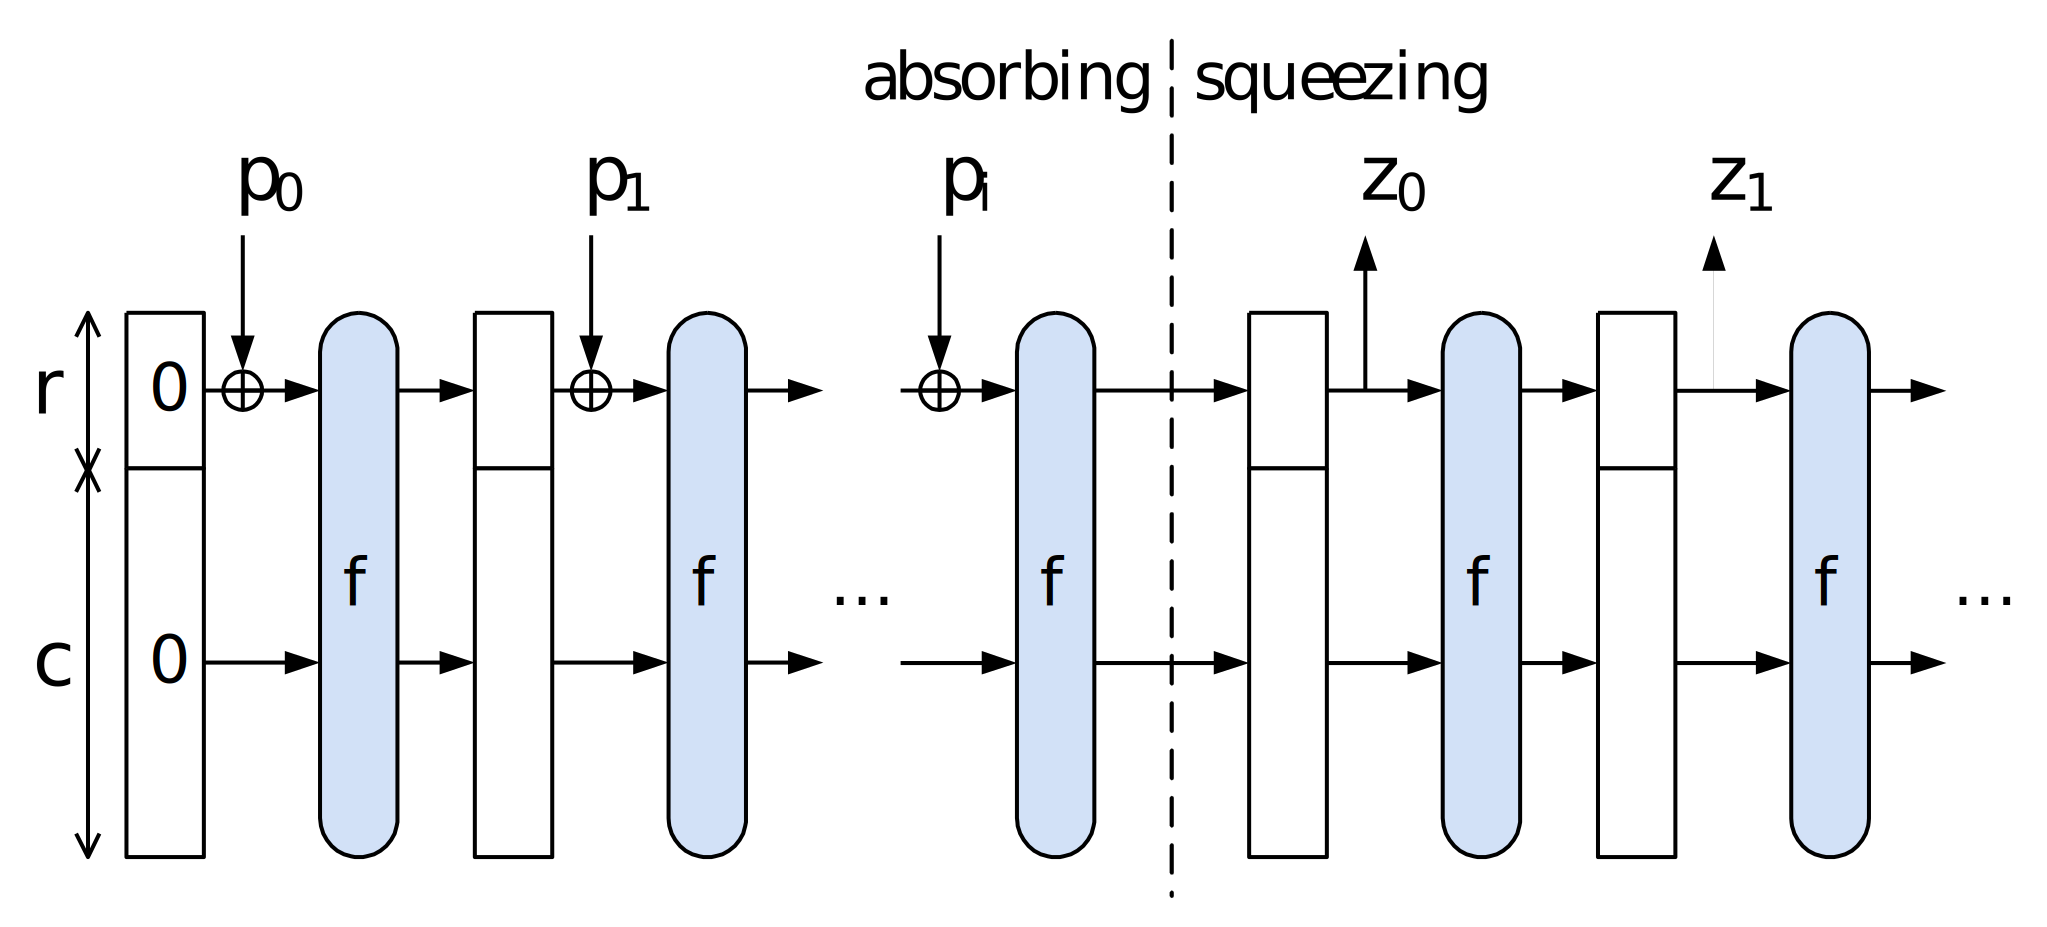
\includegraphics[width=110mm]{sponge-functions}
    \caption{Sponge function with rate $r$ and capacity $c$ absorbing a message $p$, outputting digest $z$.}\label{fig:sponge-functions}
\end{figure}

Keccak, in contrast to MD5 and SHA-1, is a sponge function, which means its internal structure is quite different from the traditional Merke-Damgård-based hash functions. Sponge functions have two phases, \emph{absorption} and \emph{squeezing}, and can be defined by their capacity $c$, the rate $r$, and their internal state size $s=c+r$, as illustrated in \autoref{fig:sponge-functions}. The higher the rate $r$, the faster messages will be absorbed and squeezed, as fewer steps through the permutation function $f$ are required. We can see that a construction like this does not enable re-construction of the internal state of the function from the bits squeezed, thus eliminating length extension attacks which make the \( h(key \| data ) \) pattern useless for Merkle-Damgård-based functions. The \(h(key \| data) \) pattern is how the Keccak designers recommend a MAC is constructed using Keccak \cite{sponge-functions}.

Keccak has an internal state size $s=1600$ bits, and can thus be fully specified by the rate. Keccak-$n$ indicates Keccak with $r=s-2n$, and an output size $n$. The strength of a sponge function is a function of its capacity, which will be 512 and 1024 bits for Keccak-256 and Keccak-512, respectively. We thus see that choosing parameters for Keccak is a speed-security trade-off, the higher the rate the better it'll perform, but at the cost of security.

While comparing these different solutions for generating MACs it's natural to also consider if there's any performance differences between them. A quick comparison of HMAC\footnote{The numbers were achieved by running the following command on the target platform: \texttt{python -m timeit -v -r 5 -n 1000 -s "msg = '10Bmessage'*10; import hmac, hashlib" "hmac.new('K'*16, msg, hashlib.sha1).digest()"}} vs. the different options for Keccak\footnote{Numbers achieved like this; substitute the 256 with 512 for the larger digest size: \texttt{python -m timeit -v -r 5 -n 1000 -s "msg = '10Bmessage'*10; import hashlib, sha3" "hashlib.sha3\_256('K'*16 + msg).digest()"}} and their performance on the target hardware is given in \autoref{tab:mac-perf-comparison}.

\begin{table}[ht!]
\caption{Performance comparison of different MAC implementations}\label{tab:mac-perf-comparison}
\centering
    \begin{tabular}{| c | c | c |}
    \hline
    \textbf{Scheme} & \textbf{Message size} & \textbf{Time} \\ \hline
    HMAC-MD5 & 100 B & 435$\mu$s \\ \hline
    HMAC-SHA1 & 100 B & 437$\mu$s \\ \hline
    Keccak-256 & 100 B & 87$\mu$s \\ \hline
    Keccak-512 & 100 B & 130$\mu$s \\ \hline
    HMAC-MD5 & 4 MB & 107ms \\ \hline
    HMAC-SHA1 & 4 MB & 169ms \\ \hline
    Keccak-256 & 4 MB & 1207ms \\ \hline
    Keccak-512 & 4 MB & 2208ms \\ \hline
    \end{tabular}
\end{table}

The rather abysmal performance of Keccak on the larger messages are not expected to be noticeable, since the underlying network is most likely going to be the bottleneck. When optimized the satellite can start sending bytes on the wire while performing the hash computation, and thus the hashing only needs to be faster than the underlying network. For the radio interface of an actual in-orbit satellite communicating over ham radio we're looking at bandwidths on the order of tens of Kbps, or likely less, which neither of the Keccak's will have any problem keeping up with. Another MAC could also be negotiated during the session establishment phase if an application in a different domain is restricted by Keccak performance. Note that one of the reasons for Keccak's poor performance on our Raspberry Pis is due to the \texttt{pysha3}-module not utilizing the optimized assembly code for ARM provided in the Keccak reference. Other implementations might have other performance characteristics; as always, benchmark if you're in doubt.

Keccak-$n$ as has a rate of \(1600-2n\), so the Keccak-256 tested had a rate of 1088 bits. Instead of MAC truncation like we're doing, this could be sped up by setting the internal Keccak sponge capacity to 128 bits and thus achieve a rate of 1472 bits, roughly 35\%  speedup. Note however that this is not supported in the \texttt{pysha3} module, as they only expose a traditional hashing interface to Keccak, and not to the underlying sponge function. Other implementations wanting to re-use the protocol, without the reference implementation provided here, are of course free to optimize this, at the cost of interoperability with other implementations.

For completeness, the current state of the art of breaking MAC-Keccak (Keccak as a MAC) is a cube attack against a reduced round (5 and 6 rounds) version of Keccak \cite{keccak_cube_attack}. The full version uses 24 rounds.


\section{Related Work}\label{sec:related_work}

This project builds mostly upon previous work done by other students working on the NUTS project, analyzing required security properties and suggesting protocols. The first of these was done by Visockas \cite{visockas} in 2011, who proposed a protocol using encryption for the uplink. Later Prasai \cite{prasai} rightfully showed in 2012 that confidentiality is unnecessary for access control, suggesting a protocol based on HMACs and sequence numbers. Later in 2012 the suggested protocol was tested on an ad-hoc radio link by Bezem and Fjellby \cite{bezem-fjellby}. In 2014 Münch picked up the task of implementing the suggested protocol \cite{marius-project}, and later trying to integrate it to the NUTS hardware \cite{marius}. However, this implementation moved away from the complexities of the sequence numbers and the problematic synchronization routines suggested previously, in favor of a system based on broadcast timestamps. In contrast to the previous work though, this work does not have a way to authenticate the downlink, and was thus not found to satisfy the desired properties of the protocol.

The protocol suggested here bears many similarities to \gls{tls}, and in particular it's datagram-based variant \gls{dtls}. TLS is the most widely deployed protocol on the Internet for secure communication, and has had years of scrutiny of both the protocol and several implementations. DTLS is very similar to it's stream-oriented sibling, sharing the same message construction and many of the same cipher suites, apart from stream ciphers like RC4. Environments with constrained resources -- like satellites and their radio links -- is exactly the motivation for standards like \gls{psk} over DTLS \cite{rfc4279}. Combining this with NULL encryption cipher suites like TLS\_ECDHE\_PSK\_WITH\_NULL\_SHA256 \cite{rfc5489} would thus yield a protocol very similar to \gls{nap}. Hence, it's worth pointing out how this would differ from our protocol.

The (D)TLS record layer adds a three byte header to it's message; one byte packet type and two bytes for the length. There's also a tailing MAC with the length being equal to the digest of the MAC algorithm, thus yielding a 20 byte MAC for SHA-1 or 32 bytes for SHA-256. The protocol suggested in this paper only has two bytes of header, and a customizable 4--32 bytes of MAC, depending on the required strength in a given deployment. Our protocol thus requires less bandwidth than its (D)TLS equivalent. Granted, using (D)TLS extensions it's possible to negotiate a truncated MAC \cite{tls-extensions} reducing the MAC overhead of (D)TLS slightly, but the MAC can only be truncated to a fixed size of 10 bytes.

It's also worth noting that DTLS implementations are not as widely available as the TLS equivalent. Only recently have popular libraries started to gain support for DTLS, but several of the most common libraries such as OpenSSL and PolarSSL does not support it yet as of yet (December 2014). Among implementations which support DTLS1.2 it gets patchy when you look for specific cipher suites supported. CyaSSL for example supports DTLS1.2, but not (EC)DHE-PSK. This is a significant barrier for utilizing DTLS1.2 for our use case, as trying to extend existing TLS libraries without prior experience from development on the libraries is non-trivial.

It must also be said that writing things from scratch and not relying on existing work seems to be the spirit in which work is done on the NUTS platform, a practice that can be defended by the project's learning goals. It's also beneficial to start fresh and not carry around on the luggage (D)TLS has carried around since its early SSL days, like the MAC-then-encrypt structure that's been the source of heaps of attacks towards TLS lately (\cite[Lucky Thirteen]{lucky-thirteen}, \cite[BEAST]{beast}, \cite[CRIME/BREACH]{breach}, \cite[POODLE]{poodle}). Note however that none of these attacks apply to an authentication-only scheme, which might be due the lesser number of deployments with such schemes, and thus limited research interest in the topic.

Future applications might want to investigate whether DTLS has reached a mature enough state to be useful and implemented in popular libraries.

\chapter{Protocol Description}
\label{chp:protocol-description}

In this chapter, version 1.0 of the proposed protocol is described in detail, along with assumptions about the environment the protocol will run in, and the intended security goals.


\section{Goals}\label{sec:goals}

The overarching goal of the protocol is to ensure that all parties participating in communication with the satellite can trust that all messages passed through the protocol were sent by another authenticated party. In other words, the satellite should only respond to commands from peers knowing a key to the satellite, and ground stations should be certain that all messages received come from the correct satellite.

The protocol will be based on clients initiating sessions with the satellite, where sessions can last as long as required by the client. Each session is authenticated with a unique session key.

Any of the parties can send an arbitrary amount of messages over a session, and both parties can send messages without any hint from the other party. It is thus possible for a server to send diagnostic data when a session is established, or a list of available actions, without a prior message from the client. This is completely up to the application protocol.

The protocol does not attempt to provide confidentiality, as there's legal restrictions for usage of encryption on ham radio frequencies \cite[article 25.2A, p.~295]{radio-regulations}.

The protocol also does not try to protect against \gls{dos}, as most deployments will be radio-based, and can thus be rendered useless by jamming the frequencies. However, DoS attacks due to resource exhaustion on any of the endpoints will be mitigated where possible.

Fragmentation and re-assembly of data is another non-goal that's delegated somewhere else in protocol stack if desired by the application. The goal is to provide a protocol similar to UDP in characteristics, but with some extra authentication features.


\section{Environment Assumptions}\label{sec:environment_assumptions}

    \subsection{Resource Constrained Server}

As the original problem description involved a satellite with heavy resource constraints, previous attempts at defining a protocol have assumed that public key operations would be too heavy in this environment, and based their authentication on lighter operations such as shared-key MACs. As shown later in this paper, this assumption does not hold for the Raspberry Pis, which can do each of the operations key generation, signing, verification and derive a shared secret, in approximately \( 5 ms \). See \autoref{chp:public-key-raspberry-pi} for more details.

Since the project is aimed at eventually being integrated onto the satellite platform, we have aimed for compatibility with the slower hardware on the actual satellite, and utilized public key cryptography only where strictly necessary, which is the master key re-negotiation phase.

Utilizing public key cryptography would mitigate the need for pre-shared secrets, and would make identity management a bit easier since each session could be identified by the public keys of the partners, instead of lower-layer addresses, but the same considerations regarding replay attacks would have to be taken. It would also be possible to recover from a loss of the private part of the key by simply generating a new pair and broadcasting the new public part, if the clients are willing to trust this new key.

For completeness we'd like to mention that utilizing public key cryptography for signing messages would make it possible for any listening party to verify that message signatures are indeed valid, and do not contain any hidden data. This is in contrast to the MAC-based design, where you'd have to know the secret key to verify the MACs, and two parties could thus claim to follow the protocol, but add hidden data in the MAC field, which would be undetectable by any other listening party.


    \subsection{RNG Reliability}

For the defined protocol to stay secure, a strong \gls{rng} is required on at least one side of the communication, preferably both. Normal computers have access to high-quality random data through either \texttt{/dev/urandom} on most \glspl{*nix} or \texttt{CryptGenRandom} on Windows. The Raspberry Pis have a \gls{hwrng} on-chip, which we assume we can trust, but the satellite does not have such a source. This source is assumed to be present and reliable, but implementation is outside the scope of this paper. For a more in-depth discussion of the \gls{rng}, see \autoref{chp:random-numbers}.


    \subsection{Error-Free Communications Channel}

The protocol assumes that packets sent and received will be error-free, and assumes the underlying layer discards packets with bit errors. In our test setup, UDP will silently discard faulty packets. It's not a problem if the underlying layer doesn't detect errors, as that will be caught in the MAC check, the only benefit of detecting it on a lower layer is if there's an interest to doing \gls{arq} to improve reliability, as NAP will drop all faulty messages without any feedback to the client.


    \subsection{Broadcast Channel}

We assume that there might be several clients and several servers communicating over the same frequencies, and that they're all in range of each other, everyone hearing all messages. This assumption is stronger than for previous projects, and introduces the demand for authentication of both sides of the communication. Previous projects were targeted directly to NUTS, in which you'd have a slightly stronger argument that the signals you're receiving actually come from the satellite as they match the satellites latency, doppler shift and position, but these are not trustworthy indicators to cryptographers. Nor do they apply in other environments where you don't have these very directional antennas, like in our test environment.


\section{The Protocol}\label{sec:the_protocol}

\begin{figure}[ht!]
\centering
\includegraphics[width=120mm]{protocol-packet-flow}
\caption{Packet flows in the protocol. \( R_a \) and \( R_b \) are nonces generated by the server and client, respectively. \( N_s \) and \( N_c \) are monotonically increasing sequence numbers, to keep each packet (and by extension, MAC) unique. Both parties possess the shared key \( K \), and use the nonces to derive a session key \( S \) after a mutual challenge-response handshake.}\label{fig:protocol-packet-flow}
\end{figure}

Here follows an overview of the different messages sent back and forth in the \acrfull{nap}. All messages follow a general format, as seen in \autoref{tab:general-packet-structure}. The most important messages and their cryptographic parameters are show in the sequence diagram in \autoref{fig:protocol-packet-flow}.

\begin{table}[ht!]
\centering
    \begin{tabular}{r | c | c | c | c |}
    \cline{2-5}
    Byte range & 0--1 & 1--2 & 2--(n-mac\_len) & (n-mac\_len)--n \\ \cline{2-5}
    Content & Type & Sequence number & Application data & MAC \\ \cline{2-5}
    \end{tabular}
    \caption{General packet structure for packet of length \( n \). Sequence numbers are not present on handshake messages. We assume for simplicity here that the sequence number can be represented as a single byte.}\label{tab:general-packet-structure}
\end{table}

The MAC field is generally computed as \( MAC_{key}(MSG\_TYPE \| MSG \ [\| OPTIONS]) \), where the key is either the shared secret \( K \) in the case of the first handshake messages, or the session key \( S \) in the case of the others. OPTIONS are used in the handshake phase to respond to challenges issued by communicating parties, which is not part of the reply. A more thorough description of all the different messages is given below.


    \subsection{The Session Key}\label{sec:session-key}

The session key \gls{kdf} used for \gls{nap} is \gls{hkdf} \cite{hkdf}, as standardized through RFC 5869 \cite{rfc5869}. The \gls{hkdf} computation involves two phases using HMAC-SHA512; key material extraction and then key expansion, with the parameters as shown in \autoref{eq:hkdf}.

\begin{equation}
    \begin{aligned}
    pseudo\_random\_key& = extract(salt, input\_keying\_material) \\
    key& = expand(pseduo\_random\_key, info, length=32)
    \end{aligned}
    \label{eq:hkdf}
\end{equation}

NAP uses the values defined in \autoref{tab:hkdf-parameters} for the different parameters.

\begin{table}[ht!]
\centering
    \begin{tabular}{| l | l |}
    \hline
    \textbf{Parameter} & \textbf{Value} \\ \hline
    input\_keying\_material & shared secret \\ \hline
    salt & \( R_a \| R_b \) \\ \hline
    info & protocol version (e.g. "1.0") \\ \hline
    length & 16 \\ \hline
    \end{tabular}
    \caption{HKDF parameter values for session key generation}\label{tab:hkdf-parameters}
\end{table}


    \subsection{Protocol Messages}\label{subsec:protocol-messages}

Here we'll take a more detailed look at the different messages. Each message sent starts with a byte indicating the type of message, optionally some more parameters, some content, and a MAC, as illustrated in \autoref{tab:general-packet-structure}. The starting byte of the message also indicates which side of the protocol issued the message, thus preventing duplicate MACs even if the content in a message from the server is identical to that of one from the client and the sequence numbers sync up. The bytes assigned to each message can be seen in \autoref{tab:protocol-messages}.

\begin{table}
\caption{Protocol messages in NAP}\label{tab:protocol-messages}
\centering
    \begin{tabular}{| l | l | p{5cm} |}
    \hline
    \textbf{Byte} & \textbf{Symbolic name} & \textbf{Description} \\ \hline
    0x00 & CLIENT\_HELLO & First message from client, with challenge to server and protocol version \\ \hline
    0x01 & SA\_PROPOSAL & Security association suggested by client \\ \hline
    0x02 & CLIENT\_DATA & Application data from the client \\ \hline
    0x03 & REKEY & Negotiate a new master secret \\ \hline
    0x04 & REKEY\_CONFIRM & Commit the new shared master key \\ \hline
    0x05--0x07e & Unassigned & \\ \hline
    0x7f & CLIENT\_TERMINATE & Client is terminating the session \\ \hline
    0x80 & SERVER\_HELLO & First response from server, responds to client challenge and challenges client \\ \hline
    0x81 & SA & Negotiated security association from server \\ \hline
    0x82 & SERVER\_DATA & Application data from the server \\ \hline
    0x83 & VERSION\_NOT\_SUPPORTED & Version suggested by client is not supported by server \\ \hline
    0x84 & REKEY\_RESPONSE & Respond to a re-key request by sending the server's public key \\ \hline
    0x85 & REKEY\_COMPLETED & Confirm back to the client that the re-keying has been committed \\ \hline
    0x86--0x8e & Unassigned & \\ \hline
    0xff & SERVER\_TERMINATE & Server is terminating the session \\ \hline
    \end{tabular}
\end{table}

There's plenty of room for expansion in the protocol, either for future standard types defined in upcoming versions or for extensions to utilize. Note that these message types are only for NAP, application-level protocols should define their own message format and use that to differentiate the different kinds of messages that might come through.

The maximum message size supported by the protocol is a function of the \gls{mtu} of the underlying transport. The protocol therefore exposes it's MTU to the application, which is defined as \( MTU_{NAP} = MTU_{T} - (5 + mac\_len) \), where the overhead added by a session is the sum of it's MAC length, the type byte and up to 4 bytes of sequence number. It's up to the application-layer protocol to perform fragmentation and re-assembly if it requires support for messages larger than the MTU of the NAP session.


        \subsubsection{CLIENT\_HELLO}

\begin{table}[ht!]
\centering
    \begin{tabular}{r | c | c | c | c |}
    \cline{2-5}
    Byte range & 0--1 & 1--2 & 2--10 & 10--18 \\ \cline{2-5}
    Content & 0x00 & Version & \( R_b \) & MAC \\ \cline{2-5}
    \end{tabular}
    \caption{Packet structure of CLIENT\_HELLO packets. Total size: 18 bytes.}
\end{table}

The first message exchanged in a session is the CLIENT\_HELLO. The version is the highest version of the protocol the client supports. The client generates a random number \( R_b \), computes the MAC as \( MAC_k(0x00 \| Version \| R_b ) \), and sends it to the master. \( R_b \) serves as a challenge to the master, to make sure we're talking to someone that legitimately knows the shared secret.

The version supported should be encoded as a single byte, with the four major bits indicating the major version, and the lower four bits indicating the minor version. 0x10 thus represents version 1.0, while 0xff is the highest supported version of 15.15. This is hopefully enough to allow the protocol to grow for quite some time.


        \subsubsection{SERVER\_HELLO}

\begin{table}[ht!]
\centering
    \begin{tabular}{r | c | c | c |}
    \cline{2-4}
    Byte range & 0--1 & 1--(n-8) & (n-8)--n \\ \cline{2-4}
    Content & 0x80 & \( R_a \) & MAC \\ \cline{2-4}
    \end{tabular}
    \caption{Packet structure of SERVER\_HELLO packets. Total size: 17 bytes.}
\end{table}

The SERVER\_HELLO is the first message from the server, sent in response to a CLIENT\_HELLO. The messages answers the client's challenge and thus proves the identity of the server, and provides a challenge to the client. Receiving this message instead of a VERSION\_NOT\_SUPPORTED also means that the server supports the version suggested by the client.

The server needs to generate an 8-byte \( R_a \) and send as a challenge to the client. The MAC is computed as \( MAC_k(0x80 \| R_a \| R_b) \).


        \subsubsection{VERSION\_NOT\_SUPPORTED}

\begin{table}[ht!]
\centering
    \begin{tabular}{r | c | c | c |}
    \cline{2-4}
    Byte range & 0--1 & 1--2 & 2--10 \\ \cline{2-4}
    Content & 0x83 & Highest version supported by server & MAC \\ \cline{2-4}
    \end{tabular}
    \caption{Packet structure of VERSION\_NOT\_SUPPORTED packets. Total size: 10 bytes.}
\end{table}

The VERSION\_NOT\_SUPPORTED message is sent by the server to the client if the protocol version given by the client in the CLIENT\_HELLO is not supported by the server. The message only contains the highest version of the protocol supported by the server. The presence of this message is necessary to prevent version rollback attacks, since if the server simply discarded unknown protocol versions, an attacker could delete all CLIENT\_HELLO messages with a strong version, thus forcing the client to re-try with a weaker version. With the presence of this message, the client can differentiate the cases where a version is unsupported, and messages are lost, and hence will not re-try with weaker versions if the first attempt doesn't generate a response.

The MAC is computed as \( MAC_k(0x83 \| version \| R_b) \). The version should be encoded using the same single-byte encoding as in the CLIENT\_HELLO.

If the client supports the version given by the server it should retry the CLIENT\_HELLO with that version.


        \subsubsection{SA\_PROPOSAL}

\begin{table}[ht!]
\centering
    \begin{tabular}{r | c | c | c |}
    \cline{2-4}
    Byte range & 0--1 & 1--(n-8) & (n-8)--n \\ \cline{2-4}
    Content & 0x01 & CBOR-encoded key-value map & MAC \\ \cline{2-4}
    \end{tabular}
    \caption{Packet structure of SA\_PROPOSAL packets. Total size: From 9 to \gls{mtunap} bytes.}
\end{table}


The \gls{sa} proposal is suggested cryptographic parameters to use for the session, and responds to the challenge from the server. A compliant server should select the union of it's own supported ciphers and the ones suggested by the client, and pick the strongest one. The client can also suggest a length to use for the MAC, which should be a number of bytes between 4 and 32. The SA\_PROPOSAL is sent as a serialized key-value mapping, serialized using \gls{cbor} \cite{cbor}, a compact binary JSON-like serialization format recently standardized by the IETF.

All parameters in the SA has sensible defaults (for the NUTS project), thus usually the client can simply submit an empty proposal, and the server will select the defaults.

\begin{table}
\centering
    \begin{tabular}{| l | l | l |}
    \hline
    Key & Type & Default \\ \hline
    mac & List of suggested MAC algorithms & sha3\_256 \\ \hline
    mac\_len & Integer in the range 4--32 & 8 \\ \hline
    \end{tabular}
    \caption{Potential parameters in the security association suggested by the client.}\label{tab:sa}
\end{table}

The current suggested protocol does not attempt to be overly compact, simply utilizing plain-text names for the protocols to use, and the keys in the mapping. This is done for readability and keeping the scope of the project manageable. If seriously bandwidth constrained a mapping between bytes and MAC algorithms could be made (and probably standardized by IANA), and a similar mapping between keys and their human readable name.

Since this is simply a key-value mapping, extending the protocol with optional parameters for encryption, extensions, timeout values, or anything else should be a simple matter.

The MAC should be computed as \( MAC_k(0x01 \| CBOR-data \| R_a) \), thus answering the challenge from the server and proving knowledge of the shared key.

An implementation of the protocol only has to support Keccak-256, supporting other MACs like HMAC-SHA256 or Keccak-512 is optional.


        \subsubsection{SA}

\begin{table}[ht!]
\centering
    \begin{tabular}{r | c | c | c |}
    \cline{2-4}
    Byte range & 0--1 & 1--(n-8) & (n-8)--n \\ \cline{2-4}
    Content & 0x81 & CBOR-encoded key-value map & MAC \\ \cline{2-4}
    \end{tabular}
    \caption{Packet structure of SA packets. Total size around 30 bytes.}
\end{table}

The \gls{sa} message from the server is the final set of parameters to use for the rest of the session. It contains the MAC algorithm and the length to use as decided by the server. To minimize ambiguity, the parameters are always sent even if just the defaults was selected. The message thus have to include at least the \texttt{mac} and \texttt{mac\_len} keys in the CBOR-encoded key-value mapping.

The MAC for this message is computed using the session key, which is derived using HKDF as described in \autoref{sec:session-key}. The length is still truncated to 8 bytes like all the other handshake messages, since the client can't extract the SA parameters from this message to determine the length before it has validated the MAC.

The size of this message depends on the textual representation of the MAC algorithm selected, and whether any extensions are used. The CBOR encoding of the key-value map for the default parameters will look like this (23 bytes):

\begin{table}[ht!]
\centering
    \begin{tabular}{c | c | c | c | c | c | c | c}
    0xa2 & 0x63 & mac & 0x68 & sha3\_256 & 0x67 & mac\_len & 0x08
    \end{tabular}
\end{table}

The first 0xa2 byte indicates a map with two values, 0x60--0x77 indicates a UTF-8 string of length 0--23, and 0x08 the integer 8. We see that the textual representation of Keccak-256 is 8 bytes, and the only part of this message likely to change much. This is also probably the shortest algorithm to be represented, as "HMAC-SHA1", "HMAC-SHA256", "sha3\_512" and the likes are all as long or longer.


        \subsubsection{CLIENT\_DATA and SERVER\_DATA}

\begin{table}[ht!]
\centering
    \begin{tabular}{r | c | c | c | c |}
    \cline{2-5}
    Byte range & 0--1 & 1--2 & 2--(n-mac\_len) & (n-mac\_len)--n \\ \cline{2-5}
    Content & 0x02/0x82 & Sequence number & Application data & MAC \\ \cline{2-5}
    \end{tabular}
    \caption{Packet structure of CLIENT\_DATA and SERVER\_DATA packets. We assume that the sequence number fits in a single byte in the figure. Total size: at least \( mac\_len+2 \) bytes.}
\end{table}

For CLIENT\_DATA and SERVER\_DATA messages, there is a field for sequence numbers. This is a an integer, encoded as a variable length quantity, meaning sequence numbers will never repeat in a single session, and can grow arbitrarily large. The encoding uses only one byte for all numbers below 127, which is probably sufficient for most sessions. Numbers between 128 and 16383 uses 2 bytes, 16834 to 2097152 uses 3 bytes, and so on. The encoding is the same as the one first used in the MIDI format, using the MSB of each byte to indicate whether there are more bytes following, thus utilizing 7 bits of each byte for the actual number. For practical considerations the maximum length for the sequence number can be limited to 4 bytes to not overflow a 32-bit integer, enabling a maximum of \( 2^{(7 \times 4)} - 1 = 268 435 455 \) messages in a session, or roughly one message per second for 8 consecutive years until you'd have to start a new session.

The MAC for these messages are computed with the session key over the entire message sent.


        \subsubsection{REKEY}

\begin{table}[ht!]
\centering
    \begin{tabular}{r | c | c | c | c |}
    \cline{2-5}
    Byte range & 0--1 & 1--2 & 2--34 & 34--n \\ \cline{2-5}
    Content & 0x03 & Sequence number & Client\_pubkey & MAC \\ \cline{2-5}
    \end{tabular}
    \caption{Packet structure of a REKEY packet. Sequence number is assumed to fit in a single byte for simplicity in this diagram. Total size: \( 34 + mac\_len \) bytes.}
\end{table}

Re-keying is done if the master key is lost or suspected compromised, and is largely equivalent to you losing the password to your email account -- you better be faster than the attacker in changing passwords, or you'll have lost your account. The same goes for the satellite, if the attacker is able to re-key the satellite, you'll be locked out with no hope of getting it back.

Re-keying works by establishing a normal session with the existing key, and then issuing a REKEY message. The REKEY message consist of an ad-hoc Curve25519 public key, and the satellite will respond with it's ad hoc Curve25519 public key. Both parties can now derive the new master key by doing a scalar multiplication of their own private key and the other party's public key. A final pair of messages is exchanged to make sure both parties did indeed arrive at the same new key, and commit the action. For the satellite, this means invalidating all existing sessions, since the compromise of the old master key means all existing sessions can be hijacked, due to the session key being derived from the master key and the two nonces, all of which are now known by the attacker.

Curve25519 is a specification of a an Edwards curve, which can be used in an elliptic curve variant of Diffie-Hellman, which was chosen for it's speed and small size of keys. Public and private keys are both 32 bytes, and the result of the scalar multiplication of the other parties public key and your own private key will be the shared secret, which is also 32 bytes. Following the recommendations from NIST for key establishment (\cite{sp800-56a}), we'll derive the new shared keying material from this shared secret, using the same HKDF construction as used in the handshake, but with different parameters. The parameter used are depicted in \autoref{tab:hkdf-rekey-parameters}.

\begin{table}[ht!]
\centering
    \begin{tabular}{| l | l |}
    \hline
    \textbf{Parameter} & \textbf{Value} \\ \hline
    input\_keying\_material & master key || session key \\ \hline
    salt & shared secret \\ \hline
    info & protocol version (e.g. "1.0") \\ \hline
    length & 32 \\ \hline
    \end{tabular}
    \caption{HKDF parameter values when generating new master secret}\label{tab:hkdf-rekey-parameters}
\end{table}

Since this operation involves public key cryptography, a note about performance is necessary. On the Raspberry Pi, using the \texttt{libsodium} library's implementation of Curve25519 we were able to perform key generation and the scalar multiplication in about \( 8 ms \), which is more than fast enough for our needs. In comparison, generating a single RSA key takes several seconds on the Raspberry Pi. This vastly superior performance is the prime motivation for elliptic curve based operations in general, and the Curve25519 specification and the \texttt{libsodium} implementations in particular. A more detailed benchmark is included in \autoref{chp:public-key-raspberry-pi}.


        \subsubsection{REKEY\_RESPONSE}

\begin{table}[ht!]
\centering
    \begin{tabular}{r | c | c | c | c |}
    \cline{2-5}
    Byte range & 0--1 & 1--2 & 2--34 & 34--n \\ \cline{2-5}
    Content & 0x84 & Sequence number & Server\_pubkey & MAC \\ \cline{2-5}
    \end{tabular}
    \caption{Packet structure of a REKEY\_RESPONSE packet. Sequence number is assumed to fit in a single byte for simplicity in this diagram. Total size: \( 34 + mac\_len \) bytes.}
\end{table}

The REKEY\_RESPONSE is the server replying to a re-key request, with its own ad-hoc Curve25519 public key. Upon receiving the REKEY message and having generated a new keypair, the server has all the components necessary to derive the new master key. It must however wait for the REKEY\_CONFIRM before performing the actual update of the new master key.


        \subsubsection{REKEY\_CONFIRM}

\begin{table}[ht!]
\centering
    \begin{tabular}{r | c | c | c |}
    \cline{2-4}
    Byte range & 0--1 & 1--2 & 2--n \\ \cline{2-4}
    Content & 0x04 & Sequence number & MAC \\ \cline{2-4}
    \end{tabular}
    \caption{Packet structure of a REKEY\_CONFIRM packet. Total size: \( 2 + mac\_len \) bytes.}
\end{table}

The REKEY\_CONFIRM serves to verify that the client and the server have negotiated the same new master key. This message is empty except for the type byte, sequence number and the MAC.

The MAC should be computed with the new master key computed using HKDF as described in the REKEY packet description.

The sequence number doesn't serve a particular purpose in preventing replays for this packet, as replaying this packet doesn't make sense anyway, but it's present to maintain consistency in the sense that every packet exchanged between the parties increases the sequence number.


        \subsubsection{REKEY\_COMPLETED}

\begin{table}[ht!]
\centering
    \begin{tabular}{r | c | c | c |}
    \cline{2-4}
    Byte range & 0--1 & 1--2 & 2--n \\ \cline{2-4}
    Content & 0x85 & Sequence number & MAC \\ \cline{2-4}
    \end{tabular}
    \caption{Packet structure of a REKEY\_CONFIRM packet. Total size: \( 22 + mac\_len \) bytes.}
\end{table}

The REKEY\_COMPLETED confirms to the client that the requested re-key operation has been completed, and a new session can be set up with the newly derived master key. The current session will be terminated, since the parties need to negotiate a new session key, but implementations are free to hide this termination and re-establishment phase from the consumer.


        \subsubsection{CLIENT\_TERMINATE}

\begin{table}[ht!]
\centering
    \begin{tabular}{r | c | c | c |}
    \cline{2-4}
    Byte range & 0--1 & 1--2 & 2--n \\ \cline{2-4}
    Content & 0x7f & Sequence number & MAC \\ \cline{2-4}
    \end{tabular}
    \caption{Packet structure of a CLIENT\_TERMINATE packet. Total size: \( mac\_len + 2 \) bytes.}
\end{table}

The CLIENT\_TERMINATE and SERVER\_TERMINATE messages are sent to indicate that the session is over. In general it would be the client that terminates the session, and it can expect to get a SERVER\_TERMINATE in return to confirm that the session has been deleted on the server.


        \subsubsection{SERVER\_TERMINATE}

\begin{table}[ht!]
\centering
    \begin{tabular}{r | c | c | c | c |}
    \cline{2-5}
    Byte range & 0--1 & 1--2 & 2--3 & 3--n \\ \cline{2-5}
    Content & 0xff & Sequence number & Reason & MAC \\ \cline{2-5}
    \end{tabular}
    \caption{Packet structure of a SERVER\_TERMINATE packet. Total size: \( mac\_len + 3 \) bytes.}
\end{table}

A SERVER\_TERMINATE is generally sent as a confirmation to a termination request from a client, but can also be sent by the server to let the client know it's session has been terminated.

The server might terminate the session if another session has performed a re-key, to let this session know that it's no use trying to continue with this session key. The client thus has to re-establish a new session to continue communication. The server might also terminate the session if it times out. The cause of the termination is sent as the reason, which is a single byte identifying these different cases, as given in \autoref{tab:terminate-reasons}.

\begin{table}[ht!]
\centering
    \begin{tabular}{| c | c |}
    \hline
    \textbf{Byte} & \textbf{Reason} \\ \hline
    0x00 & Client terminated \\ \hline
    0x01 & Re-keyed \\ \hline
    0x02 & Timed out \\ \hline
    \end{tabular}
    \caption{Different reasons given by the server for terminating a session}\label{tab:terminate-reasons}
\end{table}

The client is not expected to reply to a SERVER\_TERMINATE.


    \subsection{Message fragmenting and re-assembly}

NAP does not handle message fragmenting and re-assembly. If the underlying transport protocol has an \gls{mtu}, NAP implementations will have to be aware of this, and should raise an error condition if messages larger than the MTU is attempted sent on the channel. If the application needs to send messages larger than the underlying MTU, it needs to handle fragmentation itself. An example of how this is done is provided in one of the experiments in \autoref{chp:experiments}. Note that if this is the case, it's probably best to use RDP as the underlying transport.


\section{Formal analysis}\label{sec:formal_analysis}

To verify that our protocol adheres to certain security claims, we model it using \gls{spdl} and run it through the \gls{scyther} tool developed by Cas Cremers \cite{scyther}. The most important claim is that our protocol inhibits the non-injective property, which ensures that all messages accepted by either of the parties were accepted in the same order as in the model. This excludes an attacker from re-ordering messages sent, re-routing them to another pair of communicating parties, etc. We also claim that the derived session key will remain known only to the parties with the shared secret. The complete \gls{spdl} can be found in \autoref{chp:nuts-spdl}. Some notes to the model follow.

\gls{scyther} does not have a way to model arbitrary amounts of messages, such as repeated commands in a single session. If only the session establishment is modeled, \gls{scyther} will not be able to detect weaknesses in the rest of the protocol, such as replay attacks for command messages. To circumvent this limitation, we first model an execution of the protocol without sequence numbers (code found in \autoref{chp:nuts-spdl}), to make sure that Scyther detects the replay attack. The resulting attack graph can be seen in \autoref{fig:scyther-replay-attack}.

\begin{figure}[ht!]
\centering
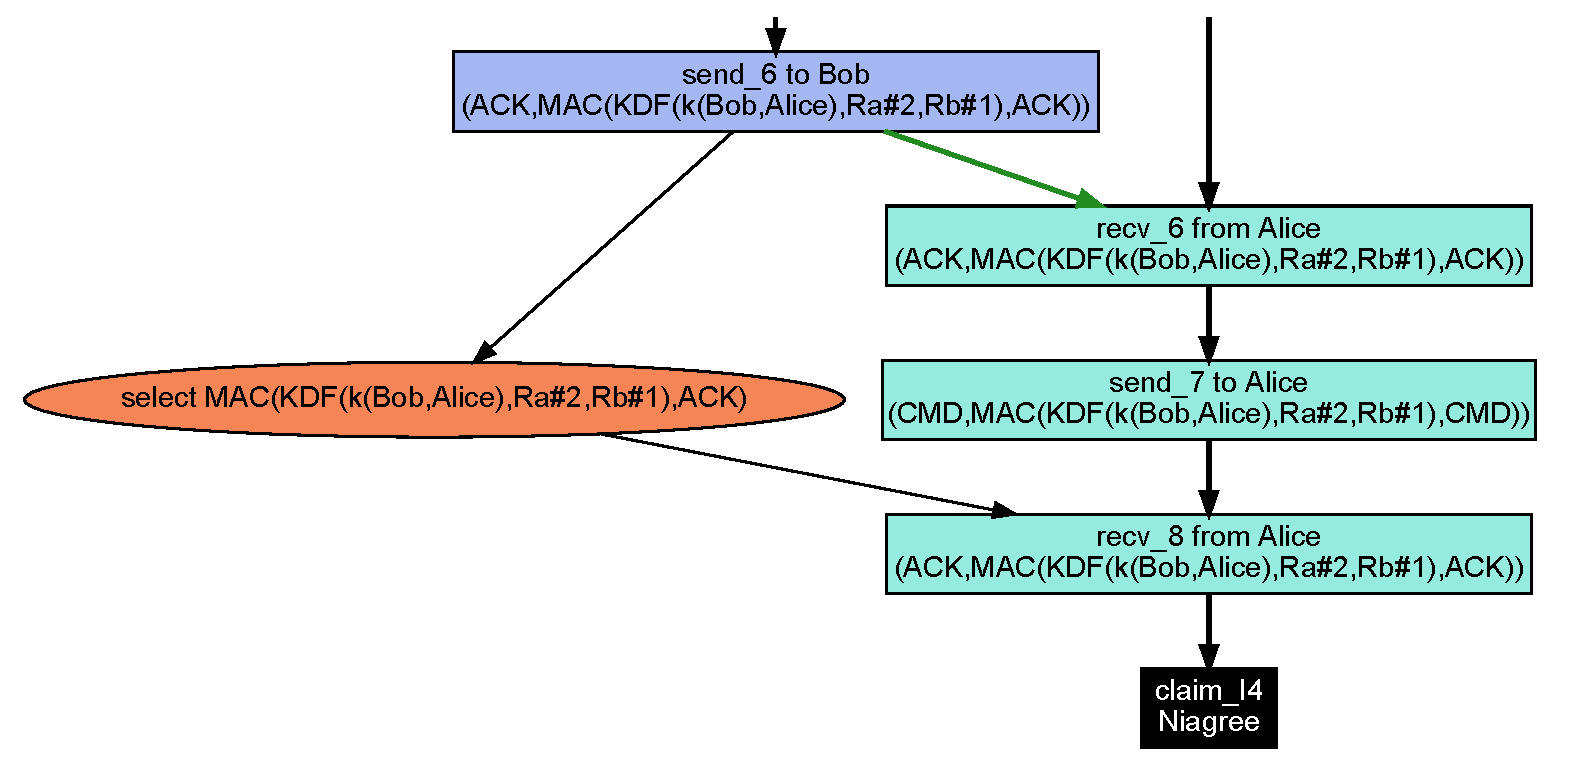
\includegraphics[width=110mm]{auth-without-seqnums}
\caption{Scyther attack graph against NAP without sequence numbers. We see that the attacker (the circle on the left) can extract the first message and send it to to Alice on the right, thus breaking the non-injective agreement.}\label{fig:scyther-replay-attack}
\end{figure}

As we now have a realistic model of how the protocol would work without sequence numbers, we can add sequence numbers to the model, and Scyther is now unable to detect any further attacks on the protocol. We then conclude that the sequence number successfully mitigate the replay attacks, if implemented correctly.

Attempts were made at modeling the re-key operations as well, but due to limitations in Scyther -- particularly no good way to model the scalar multiplication to derive a shared secret -- getting a working model would require too many hacks to simulate this operation to actually prove anything of value.


\section{Sessions}

Sessions in NAP assumes that the underlying layer provides some sort of address that can be used to associate a session to it's state and key. A session can be fully defined by it's state, the address of the other party (size depends on the underlying layer, for IPv4 this is 6 bytes for address and port) and the 16-byte session key, which amounts to a mere 23 bytes of storage.


    \subsection{Session States}

The lifetime of a \gls{session} is accurately described by a \gls{fsm}. A \gls{fsm} model of a NAP session on server side can be seen in \autoref{fig:nap-session-server}.

\begin{figure}[ht!]
\centering
    \digraph[scale=0.5]{sessionstatesserver}{
        rankdir=BT;

        inactive [label="Inactive"];
        wait_for_sa_proposal [label="Wait for SA_PROPOSAL"];
        established [label="Session established"];
        rekey [label="Re-key"];
        hidden [style=invis];

        hidden -> inactive;
        inactive -> wait_for_sa_proposal [label="CLIENT_HELLO"];
        wait_for_sa_proposal -> established [label="SA_PROPOSAL"];
        wait_for_sa_proposal -> inactive [label="Timeout", style=dotted];
        established -> established [label="CLIENT_DATA"]
        established -> inactive [label="CLIENT_TERMINATE"];
        established -> rekey [label="REKEY"];
        established -> inactive [label="Timeout", style=dotted];
        rekey -> inactive [label="REKEY_CONFIRM"];
        rekey -> established [label="Timeout", style=dotted];
    }
    \caption{Finite state machine of a server-side NAP session. In all transitions the MAC is verified, faulty messages are silently discarded. Outgoing messages are not shown.}\label{fig:nap-session-server}
\end{figure}

This model also introduces some considerations not described by the formal analysis in the previous section, most notably the timers. Having timers to automatically demote sessions from active status on inactivity is essential to avoid \gls{dos} due to resource exhaustion. Without this counter-measure, it would be trivial to capture valid \(R_b\) and \(MAC_{k}(R_b)\) pairs sent over the network, and replay them all at the same time to deplete the satellite for memory and/or storage, since it'll have to generate new \(R_a\) pairs for each connecting client. This would be roughly equivalent to the traditional SYN flood attack towards servers running \gls{tcp}\cite{syn_flood}.

Timers also protect the server against non-compliant clients not properly closing sessions, to avoid similar resource depletion. Connection timers is the satellites way to make sure that even when faced with misbehaving clients, resources are properly managed and handled. These problems could also occur due to natural causes, such as no messages coming through due to lots of noise on the radio network, or the satellite orbiting out of a reachable window. Proper resource management makes sure that the satellite can stay operational even after longer periods of time with these sorts of events happening regularly.

The corresponding FSM for a client-side session is shown in \autoref{fig:nap-session-client}.

\begin{figure}[ht!]
\centering
    \digraph[scale=0.45]{sessionstatesclient}{
        rankdir=BT;

        wait_for_server_hello [label="Wait for SERVER_HELLO"];
        wait_for_sa [label="Wait for SA"];
        established [label="Established"];
        wait_for_rekey_response [label="Wait for REKEY_RESPONSE"];
        wait_for_rekey_complete [label="Wait for REKEY_COMPLETE"];
        hidden [style=invis];

        hidden -> wait_for_server_hello [label="Sends CLIENT_HELLO"];
        wait_for_server_hello -> wait_for_sa [label="SERVER_HELLO"];
        wait_for_server_hello -> terminated [label="Timeout", style=dotted];
        wait_for_server_hello -> wait_for_server_hello [label="VERSION_NOT_SUPPORTED"];
        wait_for_sa -> established [label="SA"];
        wait_for_sa -> terminated [label="Timeout", style=dotted];
        established -> wait_for_rekey_response [label="Sends REKEY"];
        established -> established [label="SERVER_DATA"];
        established -> terminated [label="Any party terminates"];
        established -> terminated [label="Timeout", style=dotted];
        wait_for_rekey_response -> wait_for_rekey_complete [label="REKEY_RESPONSE"];
        wait_for_rekey_response -> established [label="Timeout", style=dotted];
        wait_for_rekey_complete -> terminated [label="REKEY_COMPLETE"];
        wait_for_rekey_complete -> established [label="Timeout", style=dotted];

        {rank=same; wait_for_server_hello; hidden; }
    }
    \caption{Finite state machine of a client-side NAP session. In all transitions the MAC is verified, faulty messages are silently discarded. Re-transmissions and failure handling is not shown.}\label{fig:nap-session-client}
\end{figure}

It's also worth noting that incoming packets with invalid \gls{mac} are simply ignored on both sides, and can never cause a session to respond, terminate or change state. This is essential as it's trivial to generate packets with a given source address and invalid \gls{mac} and inject into the communications channel. Allowing them to affect session state would thus be very bad practice, and open up an attack vector of very easy \gls{dos}.


\section{Extension Points}\label{sec:extension-points}

Since the parties can potentially negotiate extensions in the handshake, and there's a bunch of free messages type that extensions can use, there's plenty of opportunities for extending the protocol with whatever features are desired. Some of these are suggested below. Note that these are just suggestions, and are neither included in the sample implementation, nor standardized.


    \subsection{Session Compression Negotiation}

Depending on the deployment, it might make sense to enable support for message compression in the transport layer, similar to what TLS provides. Since the protocol doesn't provide confidentiality, there's no risk for a CRIME-style compromise of cleartext when combining compression and encryption. If implemented this should be configurable, since for some deployments another layer might already provide compression, and transport layer compression would just waste CPU cycles (like sharing JPEG images).


    \subsection{Role-Based Access Control}

For students or other people outside the core NUTS team to be able to use the satellite, to take images of stuff they want or shoot time-lapse videos or similar, a \gls{rbac} system could be implemented, to be able to give them access to certain parts of the satellite, but not others. The system should ideally work on both NAP messages, limiting access to i.e. re-keying, and application specific functions, like being able to take pictures and time-lapse videos, but not upload new code or change orientation.

The motivation for implementing this on the transport layer is that with the absence of confidentiality, passwords or access codes can't be sent in the clear, and application layer developers would have to be familiar with cryptography to be able to develop methods for doing these operations safely. Adding this functionality on the transport layer limits the number of places code that needs auditing resides, and removes the need for application layer cryptographic operations.

\chapter{Random numbers}
\label{chp:random-numbers}

High quality random numbers are essential to the security of NAP. Using the Raspberry Pi for our satellite simulator is interesting in this regard, as it includes an on-board \gls{hwrng} as provided by the Broadcom 2835 \gls{soc}. This can be compared to modern Intel CPUs providing the RDRAND\footnote{Present on CPUs from the Ivy Bridge family and onwards} instruction. Utilizing these sources for randomness should be safer than relying on a \gls{prng}, since if the state of a \gls{prng} is leaked, previous and/or future numbers generated might be predicted. With a properly implemented \gls{hwrng}, this is not possible.

However, popular adoption of the RDRAND instruction has not happened. The Linux kernel provides it's own means of sampling entropy from the environment, mixing several pseudo-random sources into an entropy pool, as provided through the \texttt{/dev/urandom} and \texttt{/dev/random} interfaces. There's been discussion in the community about this\footnote{See f. ex Bruce Schneier's blog post about it at \url{https://www.schneier.com/blog/archives/2013/10/insecurities_in.html}, and Theodore Ts'o's post at \url{https://plus.google.com/+TheodoreTso/posts/SDcoemc9V3J}}, and largely it boils down to not wanting to rely on a single source of randomness. This follows the general pattern of avoiding a \gls{spof}, which is also very much in the interest of the NUTS project. Another point to be made is that Intel has declined to share the design specifications of their \gls{hwrng}, thus denying the community the possibility to verify that the design is solid and backdoor-free. In the wake of the NSA revelations and especially the BULLRUN program\footnote{Wikipedia has a good primer: http://en.wikipedia.org/wiki/Bullrun\_\%28decryption\_program\%29}, trust in American companies claiming to provide secure solutions is failing. The same thing applies to Broadcom, which supplies the \gls{hwrng} for our Raspberry Pis.

For the NUTS project, random numbers is important, but trust in American companies is unnecessary, as the Atmel UC3-AX chip powering the satellite does not provide a \gls{hwrng}, open or otherwise. Thus the problem of generating high-quality random numbers is still an important question for the integrity of the communications channel. Luckily, the satellite has lots of hardware interfaces sampling the environment, which should provide several high-quality sources of entropy. Generating random numbers from a sensor is a matter of sampling the \gls{lsb}, before any filtering or processing has happened on the signal.

Several of the interfaces on the satellite should be excellent for this purpose, such as the two radio interfaces (background noise), the magnetometers (variations in earths magnetic field), battery voltages, CPU temperatures, camera noise, sun sensors and possibly more. A good RNG would rely on as many of these as possible.

None of these interfaces were made for being used as entropy sources though, and may be biased, in the sense that the bitstream generated by sampling the \gls{lsb} might contain more than 1s than 0s, or that some pattern might be spotted in the bitstream, such as clustering of 1s or similar. There exists several tests for testing the quality of a random bitstream, such as the NIST SP 800-90A and the FIPS 140-2 from official standards bodies, and less official tests such as the dieharder\footnote{The self-titled "Swiss army knife of random number test suites", \url{http://www.phy.duke.edu/~rgb/General/dieharder.php}} tests, which is a suite of different randomness tests. These are not adequate for testing predictability though, which is essential for any CSPRNG. Consider an RNG outputting digits of Pi. The RNG would pass all the randomness tests with flying colors, as there's no pattern or repeating element to the digits of Pi, but if an attacker observes the output, it's trivial for him to compute his own digits of Pi and search for the pattern outputted by the RNG. Once he's found where the RNG is, he can predict all future values outputted by the RNG.

It is however possible to use testing to detect catastrophic failure of the noise source, such as a stuck bit. This can be done i.e by using the Repetition Count Test or Adaptive Proportion Test from NIST SP800-90b (\cite{sp800-90b}), checking to see whether a value repeats itself too often, or whether a value appears more often than it statistically should be expected to.

However, even if the interfaces might be biased, they might still contain some actual entropy. One way to utilize them would be to guess at the entropy in the input using a pessimistic estimator, whiten the input to remove any bias, and mix it together with the other interfaces. Sum the different estimates of entropy from the inputs, and you'd have a good measure for the actual entropy of the final mixed stream of bytes. This is similar to how the Linux kernel initializes it's random pool, when a user requests random bytes, the pool content is hashed using SHA-1, and the entropy estimate is reduced with the number of bytes read. Part of the output is also mixed back into the pool.

However, our case differs from the Linux case, as the Linux kernel is written to be able to generate random numbers even in the absence of physical entropy sources, extracting entropy from other environmental sources such as timing between keystrokes, interrupts and network events. We can sample physical noise sources whenever we want, thus not having the same need for storing a pool of random data.

The problem with storing a pool of random data, is that if the pool is compromised, future output from the RNG can be predicted. This predictability compromises backwards security, the property that future output should not be predictable. This in contrast to forwards security, where previous outputs should be unguessable if one knows the current state of the RNG. Forwards security will not be compromised if the pool is leaked, as that would require successful cryptanalysis of the hash function used to generate the output from the pool, since it feeds output back into the pool.

We can thus separate two different designs here; a CSPRNG, that doesn't utilize a pool and thus have no internal state that can be compromised, and a PRNG, that utilizes a pool at the risk of its compromise. Some properties of the two approaches are shown in \autoref{tab:rng-design}.p

\begin{table}
\centering
    \begin{tabular}{| l | p{3cm} | p{3cm} |}
    \hline
    \textbf{Property} & \textbf{CSPRNG} & \textbf{PRNG} \\ \hline
    Mode of operation & Sample, whiten and mix noise sources on demand & Sample, whiten and mix noise sources on startup into a pool, hash pool contents on demand, mix part of output back into pool \\ \hline
    Speed & Depends on sampling speed and entropy of noise sources & Very fast \\ \hline
    Forwards/backwards security & Both & Only forwards, backwards only if pool is re-seeded \\ \hline
    Needs to store state & No & Yes \\ \hline
    \end{tabular}
    \caption{Different properties of a CSPRNG and a PRNG}\label{tab:rng-design}
\end{table}

For both cases, the noise sources can be treated in the same way. They need health tests, need to measure their outputted entropy, need a whitening function to remove bias, and there needs to be some way to mix the different outputs together. \cite{linux-prng-revisited} contains a good analysis of the mixing function and the estimator in Linux, and contains good points for consideration in the design of such components. RFC4086 (\cite{rfc4086}) also has a good introduction to the topic, and contains examples of both good and bad designs.

One would like to have a bit more data before choosing between the CSPRNG and the PRNG approaches, especially regarding the expected performance. However, since the performance of the CSPRNG will be a function of the estimated entropy of the sampled data, actual in-space measurements from the noise sources is necessary, as we can't tell from how they behave within Earth's atmosphere how they'll behave in space. We're not aware of any data from other in-space units sampling for randomness, and thus might have to perform these measurements ourselves.

Hence, we recommend a hybrid approach, whereas the RNG on the satellite is capable of performing both modes of operation. It could thus behave like a CSPRNG in the general case, but if performance falls below a given threshold, or noise sources fail the health tests, it might fall back to the pool-based approach, sacrificing backwards security until the noise sources return to healthy status and are able to re-seed the pool and be sampled directly. Development of such a module is recommended as future work.

\chapter{Failure Modes}
\label{chp:failure-modes}

In this chapter we will discuss different ways the protocol might fail, or situations that might compromise the integrity of the communication.

\section{Key Loss}\label{sec:key-loss}

If the secret key K is compromised you have a short window wherein you might trigger a re-keying of the satellite, comparable to how you would handle a lost password. The re-keying involves running a authenticated \gls{dh} key exchange, after completing the two-way authentication in the protocol. If the attacker who got possession of the secret key does this before you, you'll have lost your satellite. How to avoid securely store and handle keys is outside the scope of this paper, but anyone handling the master keys should be trained in managing sensitive data.

To mitigate the consequences of a master key loss, a key hierarchy should be used, where some keys can be used for operational purposes like taking pictures, and reading sensor data, while a more heavily guarded key can be used for mission-critical operations such as code upload, setting satellite orientation, resetting subsystems, re-keying, etc.

If a session key is lost, the potential consequences depend on whether a key hierarchy have been implemented or not. If role-based access control is implemented and the session key is unprivileged (i.e. can not perform a master re-key) it doesn't affect any of the other running session, previous or upcoming, as the session key is only dependent on \( R_a \) and \( R_b \) and the shared secret, and not on any previous keys. If it's an unprivileged session and you still have the key, you'd send a \texttt{CLIENT\_TERMINATE} for the server to quit the session and invalidate the session key. If you've lost the session key, you should start a new one with a privileged key and run a re-key to invalidate all existing sessions. If the session is privileged it's equivalent to loosing the master key, and your handling of the issue should be the same. This is why more work into separating normal usage from administrative use like re-keying should be done, with e. g. role based access, as briefly discussed in \autoref{sec:extension-points}.


\section{Invalid MAC Computations}\label{sec:invalid-mac}

If the server or client receives a message with an invalid MAC there's a couple of different things that could have caused this:

\begin{itemize}
    \item Message corruption not detected by the CRC32 on the underlying layer
    \item Client failed to use the correct MAC function as negotiated during the handshake, or derived a faulty session key
    \item Someone is sending bogus messages without knowing the secret key and/or the protocol
\end{itemize}

In all cases, the server should simply ignore the message as it has no way to differentiate the different situations. All of these can also occur on the client side, and the mitigation is the same, ignore the message and wait for one with a valid MAC.


\section{RNG Failure}\label{sec:rng-failure}

Much of the security of the protocol hinges on the strength of the random number generators on both sides of the communication. However, the most crucial one is the one residing on the satellite side. If the client has a faulty RNG and sends the same \( R_b \) twice, he has no guarantees that the reply comes from the actual satellite, as an attacker might have intercepted a valid reply to this challenge previously, and can respond with the same \( R_a \) and thus the same signature that the legitimate satellite used last time this \( R_b \) was used. The session key derived would be the same as last time, since the session key only depends on the shared key, \( R_a \) and \( R_b \). The attacker won't know the actual session key, but would be able to replay the satellite messages from the previous session.

If the satellite were to re-use a previous \( R_a \), you'd get a similar but mirrored attack vector. An attacker could re-send a previously sent \( R_b \) with a valid signature, get the same response from the satellite as last time, which means that the session key will be the same. He can now replay all the messages the client sent in the previous session. The attacker can not change the master key in this attack, since the key exchange involves a secret part not sent in the clear, without which the attacker would not be able to derive the new key, or confirm the key exchange, since the satellite will require a confirmation on the new key before completing the change.


\section{Replay Attacks}\label{sec:replay-attacks}

The only way for someone not knowing the shared secret to get any interaction with the satellite is to replay a previously sent message by a legitimate client. If a previous CLIENT\_HELLO is replayed, the attacker will get a valid reply from the server, but will be unable to generate a valid signature for the SA\_PROPOSAL message that should follow.

If the attacker tries to replay a CLIENT\_DATA message, as long as the satellite has received the message previously it will discard the message since the sequence number doesn't match what the satellite is expecting.

If the server hasn't processed the message yet, there's a possibility the attacker could affect the application. This could happen if the client sends a valid message, but the server is being jammed by an attacker that also intercepts the client's message. The attacker could now be the first one to send the message, and could get a reply from the server. He could also jam the client, keeping the client in the dark about the server's response to the attacker's message. However, the message will be one the client intended to send in the first place, but could be time-shifted by the attacker. Assuming the presence of a clock on both sides, an application could mitigate this by adding timestamps to timing-critical messages, and thus rejecting out of date messages. Each application protocol would need to specify their requirements in terms of clock accuracy and allowed window of execution.

No mitigation for this attack will be included in the proposed protocol, as we consider it to be the responsibility of the application-layer protocol to do a risk-assessment of whether this is something worth mitigating. Note also that if the client sends another command that is received by the server, it will invalidate the attacker's message. This works since the server now expects a sequence number great than the one that's in the message the attacker possesses.


\section{Denial of Service}

It's hard to prevent \acrfull{dos} for a service running over a radio interface, since it's a shared medium and it only requires one person to fully jam the interface for all other participants. This is in contrast to the wired Internet, where the backbone has vastly more capacity than what any single user has through her connection, and thus any effective \gls{dos} on the Internet has to be a \emph{Distributed} DoS (DDoS), where several users team up to join the strength of their connections. The users behind the connections might be unaware of the attack, as they might have had their computers get infected by a virus, and is part of botnet.

Migrations for DDoS is to some extent possible on the Internet though, since many attacks rely on spoofing the source IP. The service can thus verify that there's an actual user behind that IP, by issuing a challenge that needs to be responded to before the server will invest any resources in answering the request.

This mitigation technique is not possible over a radio link though, since there's no routing and anyone can claim any address they want. Thus, if an attacker captures a valid $R_b$ and \( MAC_k(R_b) \) pair, he can issue this from several addresses to force the server into verifying the MAC for all of the requests, generate an $R_a$ and allocate a session. The attacker will be unable to send any more messages to any of the sessions, but can create as many sessions as he desires, and thus potentially exhausting the memory of the server. The mitigation for this is to have low timeout values for the handshake messages, and longer timeouts for established sessions. This makes sure that the server discards the stuck-in-handshake sessions faster than the attacker can create them.

Timeout values would need to be configured for each underlying transport, for UDP-based environments one second (or potentially even lower) timeout should be enough to allow legitimate requests to establish a session without troubles. The same timeout value -- or slightly higher, to allow more room for the public-key cryptography -- is recommended for the re-key related messages as well. How long established sessions can stay alive without a heartbeat can easily be several hours or even days or weeks, as long as the server has enough memory to store the state of all the sessions that might appear over the period.


\section{Power Analysis}

\begin{figure}[ht!]
\centering
    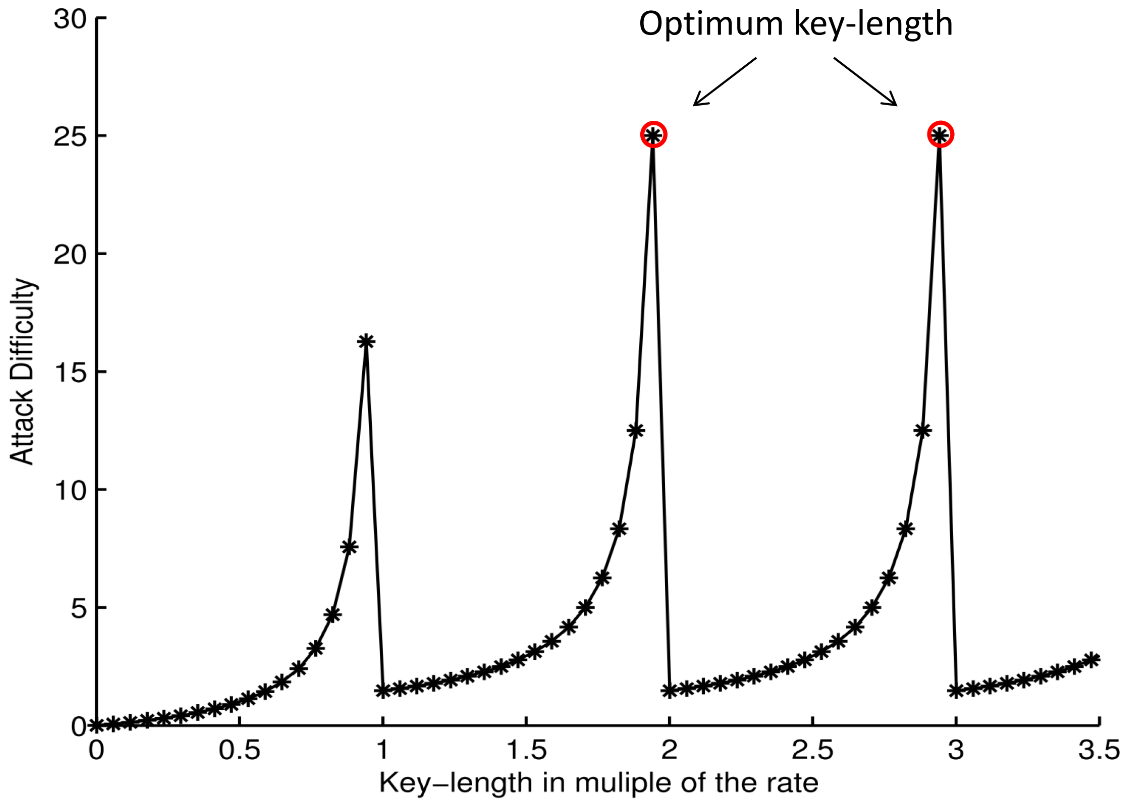
\includegraphics[width=110mm]{optimum-key-length}
    \caption{Optimal key lengths for MAC-Keccak. Illustration by Taha and Schaumont (\cite{keccak_side_channel_analysis})}\label{fig:optimum-key-length}
\end{figure}

Taha and Schaumont performed a side-channel analysis of MAC-Keccak in 2013 \cite{keccak_side_channel_analysis}, concluding with a recommended key size of \( 2*rate-1 \) to make side-channel analysis as costly as possible. The relationship between key size and cost of performing a side-channel attack is depicted in \autoref{fig:optimum-key-length}. This implies that the optimum key size for MAC-Keccak is 2175 and 1023 bits, for Keccak-256 and Keccak-512 respectively. These key sizes are significantly larger than the ones we're using in NAP, which means that a side-channel attack against the protocol using power analysis might reveal the key used for MAC computation if a sufficient amount of power traces are acquired. From the analysis by Taha and Schaumont, 5000 power traces yielded close to 90\% chance of recovering 320-bit keys against MAC-Keccak with rate 1088. Thus we can only assume that recovering our 128-bit session keys requires far fewer traces.

We're not trying to mitigate side-channel attacks in this version of the protocol, partly due to the increased storage cost of bumping the key size, and that the attack can be mitigated by physically securing the computers of the communicating parties. If a deployment of \gls{nap} can not physically secure the communicating computers, the attack can be made costlier by implementing a version of \gls{nap} with larger key sizes.

Using power analysis it's also possible to perform a timing attack against the MAC check against a naïve implementation, if the implementation does a direct string comparison of the expected MAC and the given MAC. The fault here lies in the fact that the naïve comparison will terminate on the first differing byte, thus leaking key-related data onto a side channel (time). The attacker could then guess on the first byte of the MAC, and the power analysis will reveal a slightly earlier return to idle if the guess was wrong, compared to if it was right. Thus, in 256 guesses he'd know the first correct byte of the MAC for his message. He can now continue on to the next byte, completing the entire MAC in \( 256 \times 8 = 2048 \) guesses. The sample implementation is not vulnerable to this attack, as it uses a constant-time comparison of the MACs. Note that this attack is not feasible without the power traces, as NAP doesn't give any reply to MAC failures, and thus it's not possible to profile the different guesses.

\chapter{Experiments}
\label{chp:experiments}

In this chapter the sample implementation is introduced, we'll take a look at the test environment, and present the results.


\section{Implementation}\label{sec:implementation}

    \subsection{Application Programming Interface}

The sample implementation weighs in at about 1000 lines of code, and was thus consider a bit too heavy to include directly in this paper. For that reason we'll instead focus on how an application would use the \gls{api} provided. The complete source code, with examples and tests, can be found at \url{https://github.com/thusoy/nuts-auth}.

The Python implementation exposes two different objects to the consumer of the API, a \texttt{channel} and a \texttt{session}. The \texttt{channel} is the underlying transport, which is pluggable. Using the \texttt{channel}, the application can either call \texttt{.connect(address)} to initialize a new session with a server, or call \texttt{.listen(address)} followed by \texttt{.receive()} to act as a server. Note that the current implementation does not allow the server to send a message to the client until it has received one, but this is just a limitation in the implementation, not in the protocol itself.

The sample implementation provides a UDP channel and an in-memory channel for testing, running the protocol over a custom transport only requires implementing three methods for binding, sending and receiving on a given address. The UDP implementation is provided to demonstrate how easy it is to implement a custom transport, see \autoref{udp-auth-channel}. Please note the code given in this chapter does not perform any error handling that you would do in a real application, to keep the examples concise.

Note also that timeouts are not yet being handled in the given python implementation, hence a lost packet might leave a session unusable, and will not be garbage collected by the server. It does time out if nothing is received on the channel though, as shown in the \texttt{UDPAuthChannel} implementation.

\begin{lstlisting}[caption=UDPAuthChannel Code, label=udp-auth-channel]
class UDPAuthChannel(AuthChannel):

    #: The maximum size of packets sent and received on this channel
    mtu = 4096

    def __init__(self, *args, **kwargs):
        super(UDPAuthChannel, self).__init__(*args, **kwargs)
        self.sock = socket.socket(socket.AF_INET, socket.SOCK_DGRAM)
        timeout = kwargs.get('timeout', 2.0)
        self.sock.settimeout(timeout)

    def listen(self, address):
        self.sock = socket.socket(socket.AF_INET, socket.SOCK_DGRAM)
        self.sock.bind(address)

    def send_data(self, data, address):
        self.sock.sendto(data, address)

    def read_data(self):
        data, sender = self.sock.recvfrom(self.mtu)
        return data, sender

    def tear_down(self):
        self.sock.close()
\end{lstlisting}

The \texttt{address} parameter to \texttt{.listen()} and \texttt{.send\_data()} can be whatever is needed by the underlying transport, the only requirement is that it uniquely identifies the session. This is because this is used by the channel to track the different sessions. For the \texttt{UDPAuthChannel} the address will be a tuple \texttt{(IP-address, port)}.

The first example of the application code is the client code as seen in \autoref{lst:nap-client-hello}. It uses context managers to automatically terminate the session and free any resources used by the channel when the exiting the block. This is a simple "Hello, world" application, where the client and server exchange pleasant greetings before terminating the session.

\begin{lstlisting}[caption=NAP Client Code, label=lst:nap-client-hello]
channel = UDPAuthChannel('/path/to/keyfile')
with channel.connect( ('10.0.0.1', 8001) ) as session:
    session.send('Hello, space!')
    msg = session.receive()
    print('Received from %s: %s' % (msg.sender, msg))
\end{lstlisting}

The corresponding server application is quite similar, and is given in \autoref{lst:nap-server-hello}.

\begin{lstlisting}[caption=NAP Server Code, label=lst:nap-server-hello]
channel = UDPAuthChannel('/path/to/keyfile')
channel.listen( ('10.0.0.1', 8001) )
while True:
    msg = channel.receive()
    print('%s said: %s' % (msg.sender, msg))
    channel.send('Hello, world!', msg.sender)
\end{lstlisting}\label{code:nuts-server}

The session is the object the client-side code will interact with the most, which is used for sending, receiving, terminating and re-keying. The server can access the session through the \texttt{msg.session} attribute to perform the same actions. The message object returned from both \texttt{channel.receive()} and \texttt{session.receive()} is the same class. It provides access to the address of the sender through the \texttt{msg.sender} attribute. If you just print it you'll get the only the data sent.

A slightly more comprehensive example application has also been tested, where the client fetches images taken by the server. The images taken by the camera module we have produces 180--230kB JPEGs, which do not fit within a single message -- recall from \autoref{udp-auth-channel} that we've set an MTU for the UDP transport of 4kB. We've thus invented an ad-hoc re-assembly protocol for the application, where the number of messages that's going to be sent will be sent in a single message first, and then the client can expect to read that many messages from the session. The resulting client code is given in \autoref{lst:nap-client-image}.

\begin{lstlisting}[caption=Client Re-assembling Image Data, label=lst:nap-client-image]
channel = UDPAuthChannel('/path/to/keyfile', timeout=4)
with channel.connect( ('10.0.0.1', 8001) ) as session:
    session.send('Take pic!')
    msg = session.receive()
    num_chunks = int(msg)
    with open('latest_img.jpg', 'wb') as img_fh:
        for i in range(num_chunks):
            chunk = session.receive()
            print('got chunk %d of %d' % (i + 1, num_chunks))
            img_fh.write(chunk.msg)
\end{lstlisting}

The server code now needs to add the code to actually take the picture as well, and then perform the fragmenting. Note that the image never touches the filesystem on the server, it's captured and sent directly from memory before being discarded. Code is given in \autoref{lst:nap-server-image}.

\clearpage

\begin{lstlisting}[caption=Server Fragmenting Image Data, label=lst:nap-server-image]
def take_single_picture():
    # Create an in-memory stream
    my_stream = io.BytesIO()
    with picamera.PiCamera() as camera:
        camera.start_preview()
        # Camera warm-up time
        time.sleep(2)
        camera.capture(my_stream, 'jpeg')
    my_stream.seek(0)
    return my_stream.getvalue()

def ceildiv(dividend, divisor):
    return (dividend + divisor - 1) // divisor

channel = UDPAuthChannel('/path/to/keyfile')
channel.listen( ('10.0.0.1', 8001) )
while True:
    msg = channel.receive()
    print('%s said: %s' % (msg.sender, msg))
    img = take_single_picture()
    num_chunks = ceildiv(len(img), msg.session.mtu)
    channel.send(str(num_chunks), msg.sender)
    for i in range(num_chunks):
        chunk = img[i*msg.session.mtu:(i+1)*msg.session.mtu]
        print('Sending chunk %d of %d' % (i + 1, num_chunks))
        channel.send(chunk, msg.sender)
        time.sleep(0.1)
\end{lstlisting}

    \subsection{Tests}

More than 80 test cases have been developed, and comprehensively tests the implementations handling of faulty MACs, malformed packets, replays, and out-of-order protocol execution. The code is hosted in a repository on GitHub\footnote{Repository can be found here: \url{https://github.com/thusoy/nuts-auth}}, and all tests are run by Travis CI\footnote{Travis CI is a free, continuous integration system} on both Python 2 and Python 3 for every commit to the repository. This makes it easier to collaborate on the development, as external developers more easily can verify that they didn't break anything through their changes.

What is not being tested in the current implementation are issues related to timing and timeouts, as there was no time (no pun intended) to implement and test this functionality in this project. If the test setup is utilized in TTM4137 hopefully someone will step up and contribute a fix for this.

Since this is network-facing code it should also have been fuzz tested, which could catch errors that the test cases missed.


    \subsection{Key management}

Naturally, keys needs to be stored securely on the devices. In the case of the NUTS satellite, redundant copies should be stored to try to avoid key loss in case of bursts of radiation invalidating parts of the memory. For the NUTS case though, securing access to the keys is not a concern, as we're assuming no one bothers to try to physically try to extract keys from a CubeSat in orbit. This is in contrast to our Raspberry Pi setup, where physical access is much simpler, and radiation is a non-issue. If we were deploying a production application on a similar setup, we'd probably encrypt the memory cards to make sure the keys cannot simply be extracted by putting the memory card into another computer and reading them out from the filesystem.

To make it possible for sessions to perform a re-key operation the key should not be hard-coded into the source code, but would preferably reside on some writable medium, such as a file on disk. This ensures that the new key is persisted between executions of the protocol. This file-based approach is how the sample code handles the issue.


\section{Test setup}\label{sec:test_setup}

\begin{figure}[ht!]
\centering
    \begin{subfigure}{.5\textwidth}
        \centering
        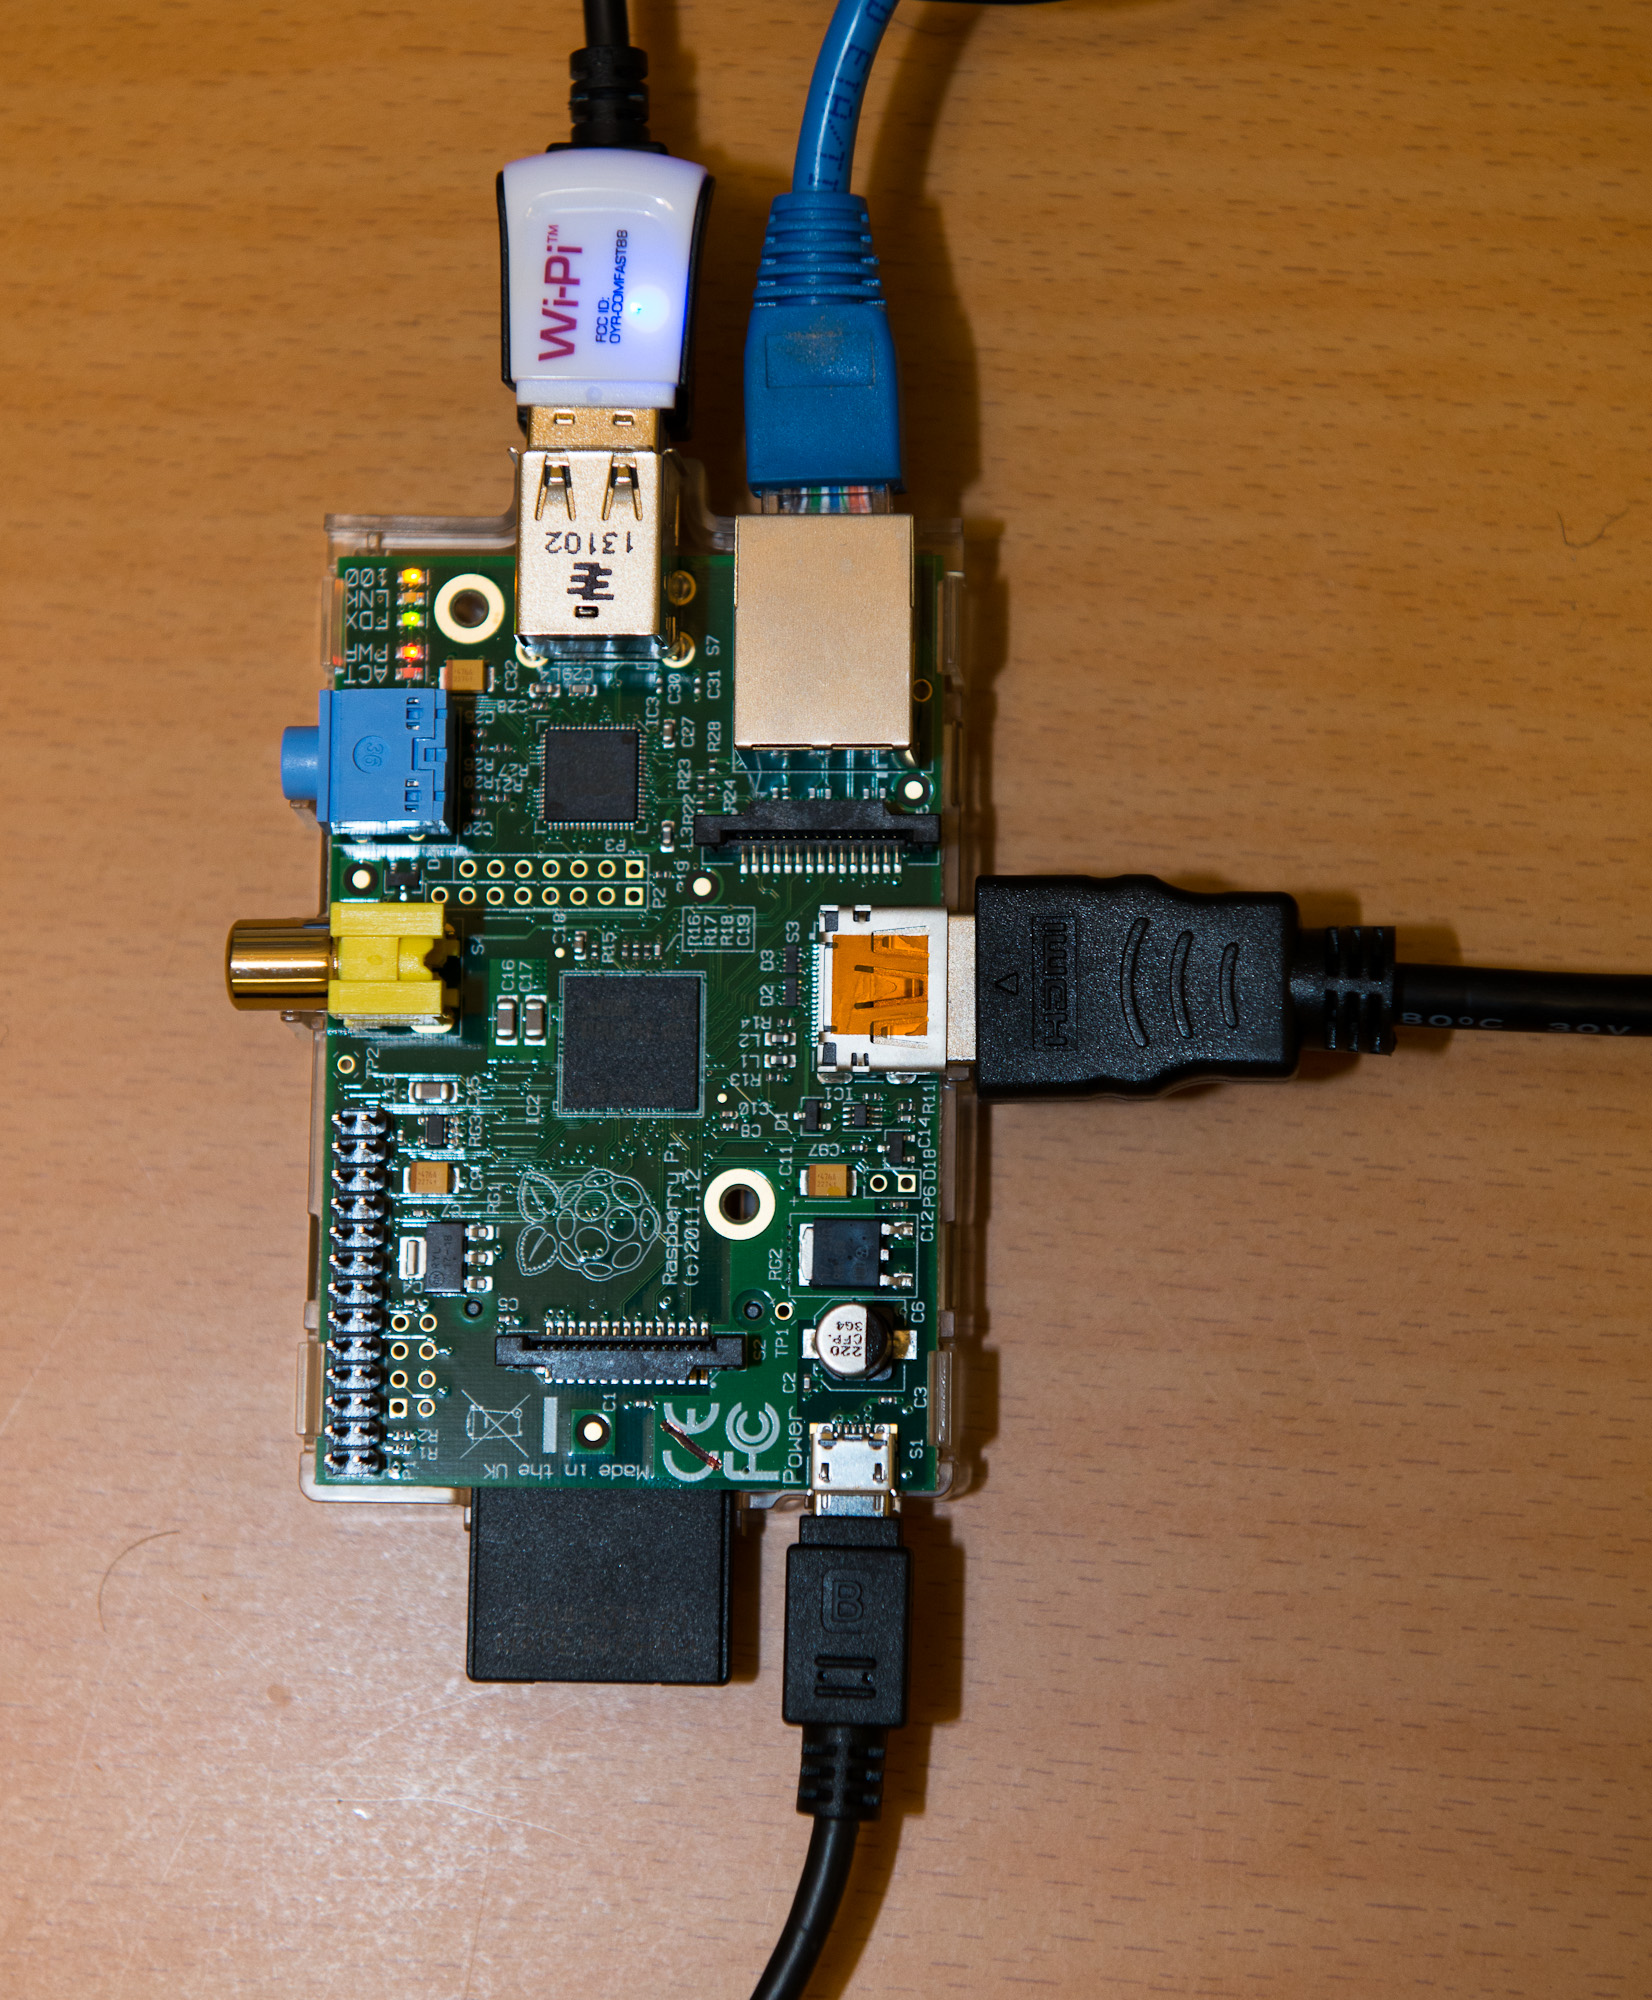
\includegraphics[width=.7\textwidth]{groundstation}
        \caption{The ground station}\label{fig:ground-station}
    \end{subfigure}%
    \begin{subfigure}{.5\textwidth}
        \centering
        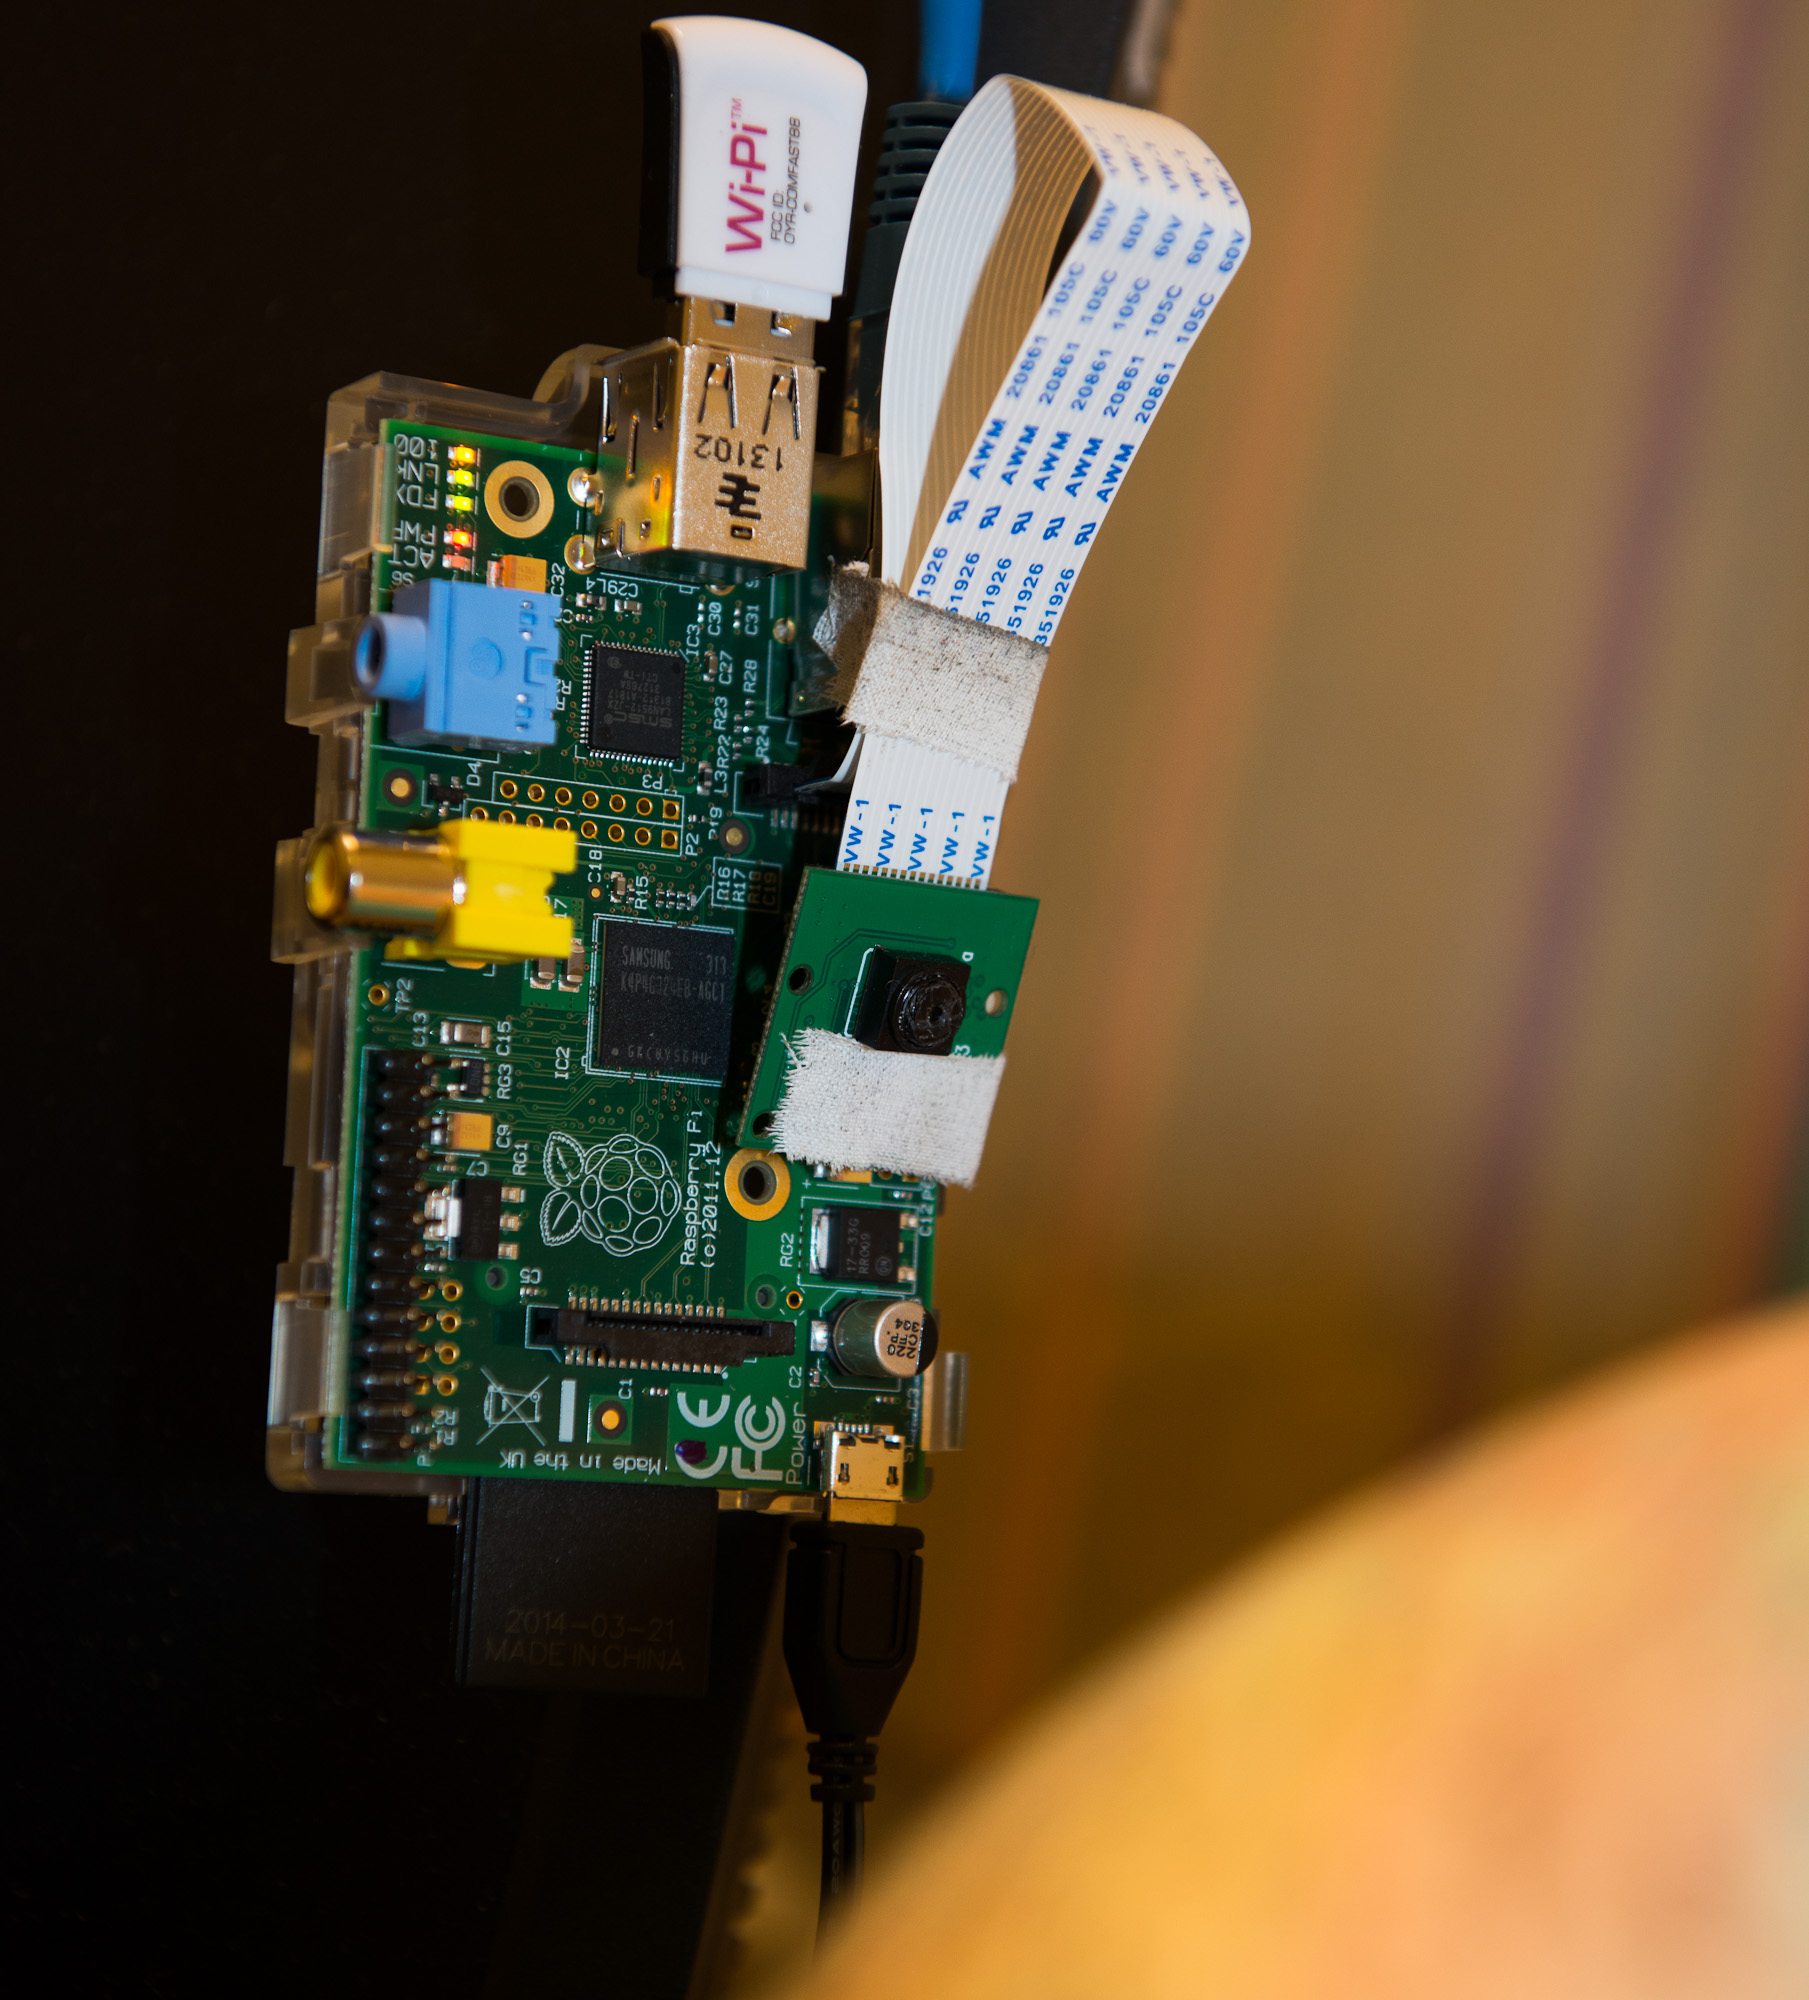
\includegraphics[width=.7\textwidth]{satellite}
        \caption{The satellite}\label{fig:satellite}
    \end{subfigure}
    \caption{The two Raspberry Pis used in the test environment}\label{fig:raspberrys}
\end{figure}

To test the code in a real environment with package loss and propagation delays, we set up a system with two Raspberry Pis, communicating over an open Wi-Fi connection. Additionally, the server was equipped with a camera, to generate payloads to send to the client. The following hardware was used:

\begin{itemize}
    \item 2 $\times$ Raspberry Pi model B
    \item 2 $\times$ Element14 Wi-Pi USB Wi-Fi dongle
    \item Element14 Raspbery Pi 5MP Camera Board
\end{itemize}

There was also one globe involved, to simulate the server being in orbit. The wireless network was hosted on the server by \texttt{hostapd}, and the server also ran a DHCP server using \texttt{dnsmasq}. Both Raspberry Pis were running Raspbian Wheezy. Both of the Raspberry Pis were like you can tell from \autoref{fig:raspberrys} also connected by Ethernet. This was merely for control purposes, to make it possible to SSH into the devices to add the code and start the tests. You can also see that the client has a HDMI connection, this was used to display the downloaded images on a monitor, as demonstrated later in \autoref{fig:test-environment}

It must be said that the code does not have to be run over Wi-Fi, it might be just as interesting for students studying the protocol to try to mount a wired \gls{mitm} attack. This could be done by utilizing a computer with two wired Ethernet interfaces, and gives you the possibility to delay packets, re-order them, drop a select few, etc. Eventually, this computer in the middle could just be used for monitoring, following the packet flow between the client and the server in real-time to better understand the protocol.


\section{Results}\label{sec:results}

The examples mentioned here run successfully in the test environment. The following is a "satellite image" taken by the server "in orbit" over Japan (\autoref{fig:test-environment}, extracted by the client using the re-assembly code given in \autoref{lst:nap-client-image}.

\begin{figure}[ht!]
\centering
    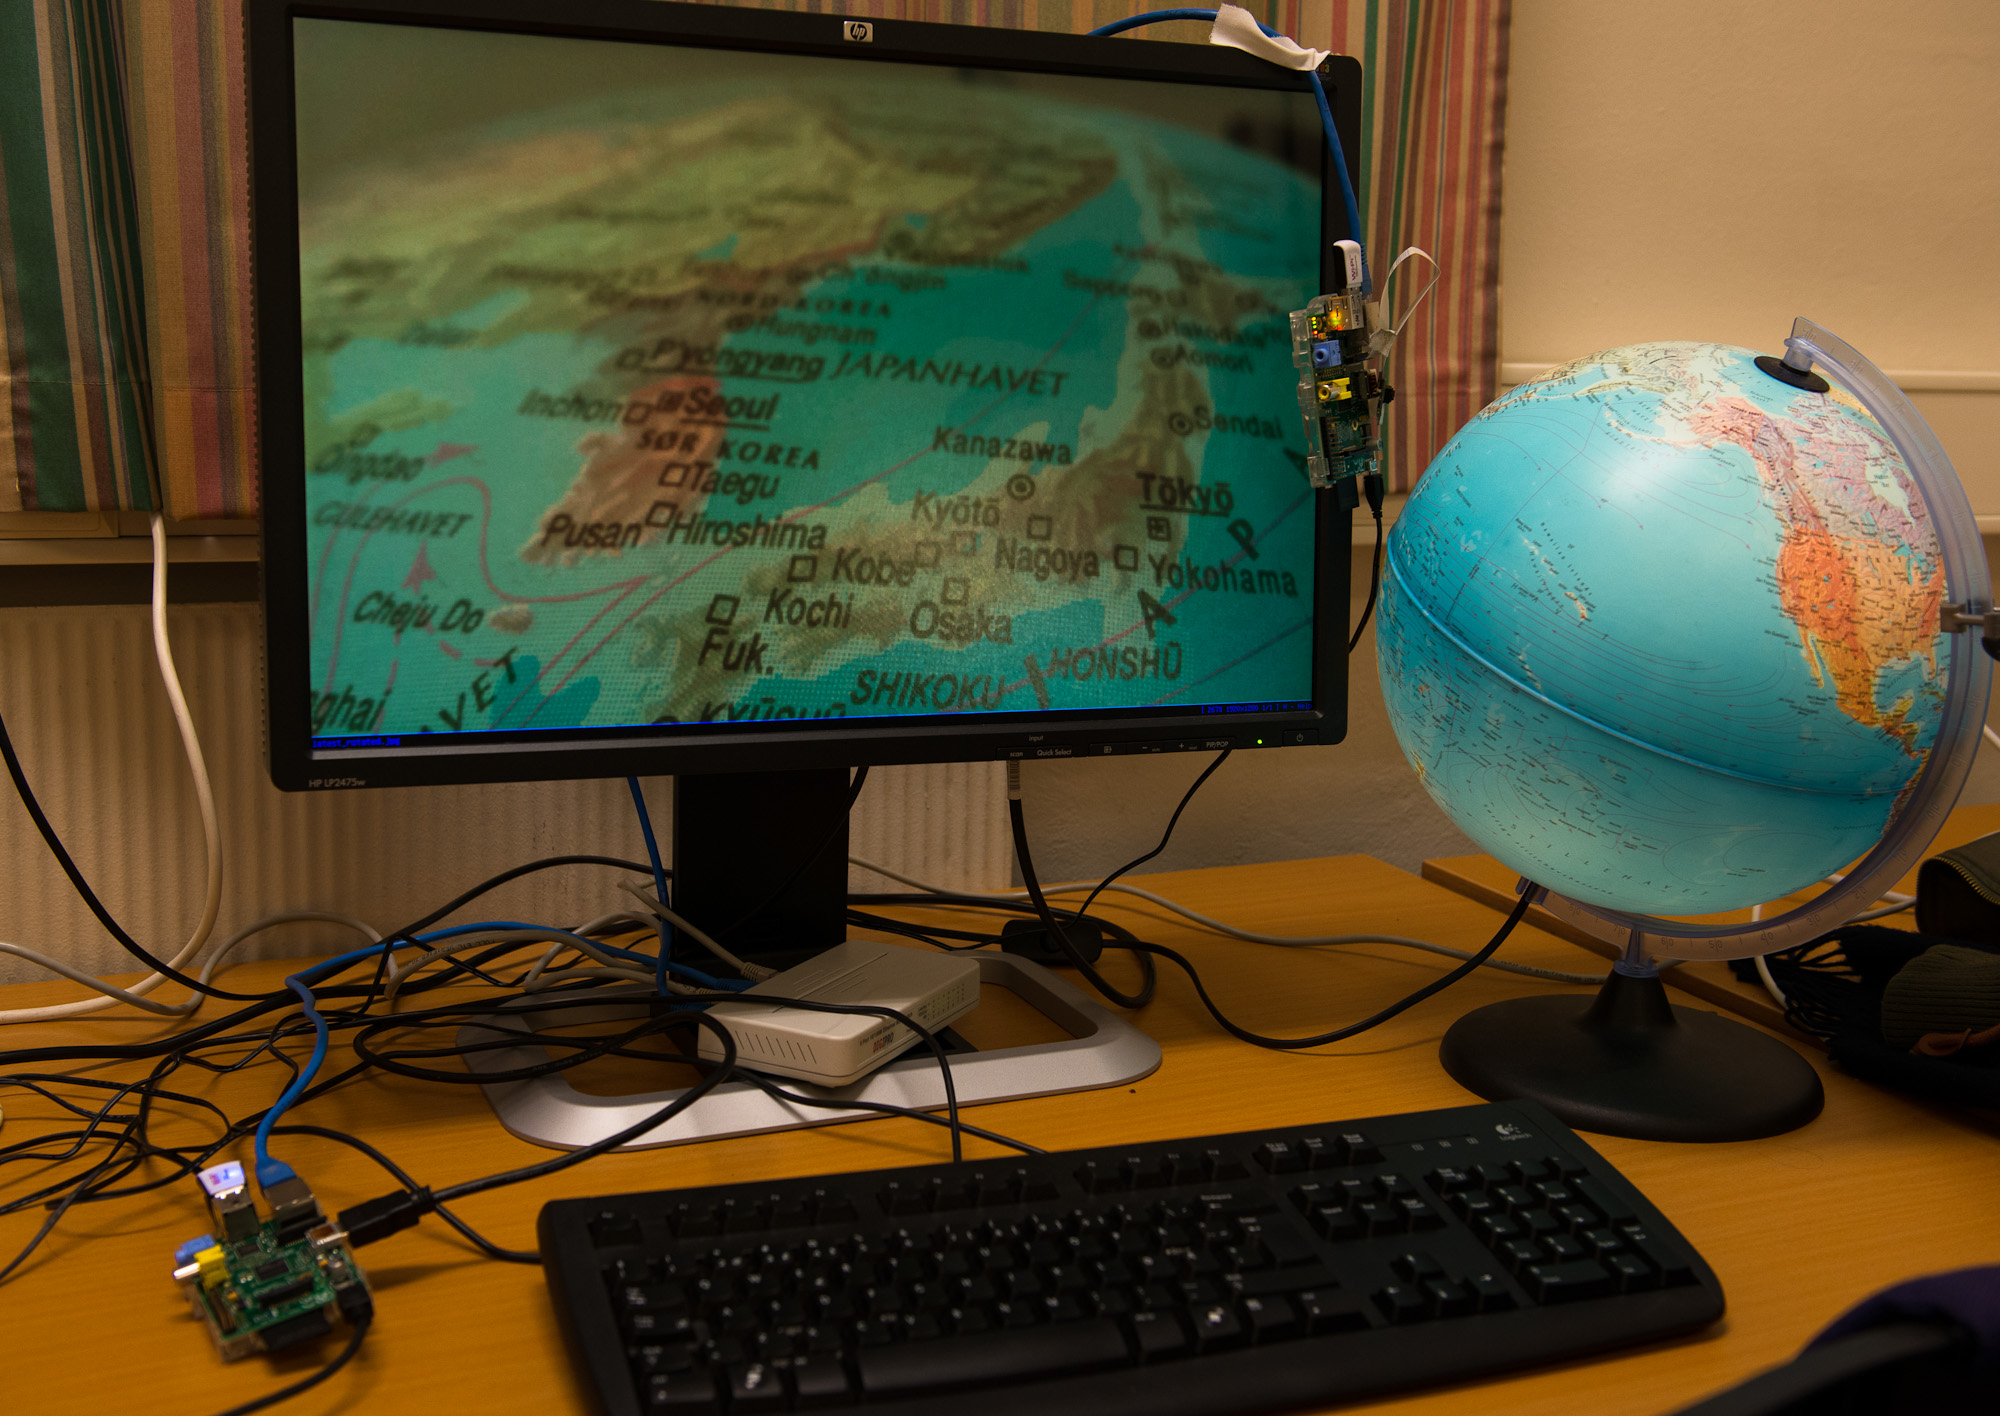
\includegraphics[width=110mm]{test-environment}
    \caption{The client displaying an image it just downloaded and re-assembled from the satellite}\label{fig:test-environment}
\end{figure}

There were some problems with executing the examples in the test environment, but the problems were not related to our code, which was frustrating. It turned out hard to configure the wireless adapters without them sporadically loosing their IP after some time. This happened irregularly on both devices, requiring either restarting the wireless interface or a full restart of the unit to get things back into a stable state. It might be that stable connectivity is more than what can be expected from a small computer costing around 200 NOK over a wireless dongle in 2014, but it was certainly worse than expected. The stability issues might be due to the wireless network being hosted on one of the Raspberry Pis, which have very limited power usage due to them being run over USB power, so it might be that the stability would have been better with a dedicated router.

\chapter{Conclusions and Future Work}
\label{chp:conclusions}

\section{Concluding Remarks}\label{sec:conclusions}

The sample implementation ended up being around 1000 lines of code, and thus considered to be a bit too big to be included in the appendices. The complete code can be browsed online, at \url{https://github.com/thusoy/nuts-auth}. It has been successfully tested between two Raspberry Pis communicating over wireless UDP, and the protocol doesn't stumble on lost messages or faulty MACs.

The code is thus ready to be utilized in the TTM4137 Wireless Network Security lab, where students can study it to understand the concepts of secure protocols, and to try to find any implementation bugs or holes in the specification that allows the protocol to be broken.


\section{Future Work}\label{sec:future_work}

Since projects like these are never completed, but merely continue evolving, there are a couple of points future projects could look into.

    \subsection{C Implementation}

To run the protocol on resource-constrained hardware like the NUTS satellite, a C implementation needs to be developed. It's not expected to be much faster than the Python implementation as all the heavy cryptographic operations in the Python code is performed by C code already, but the complete C implementation is still needed since operating systems like FreeRTOS doesn't support higher-level languages like Python.


    \subsection{Satellite RNG}

The NUTS satellite does not have access to a \acrfull{csprng}, which is a requirement for secure operation of NAP. See \autoref{chp:random-numbers} for a deeper discussion about this issue.


    \subsection{Fuzz-testing Final Implementation}

When the C implementation is completed, the entire protocol stack should be fuzz tested to try to iron out errors from malformed input packets. The upper layer protocol could also be tested for malformed messages sent by legitimate users, which could be a result from session hijacking or an error in the sending program.


    \subsection{Resistance to Power Analysis}

As we saw in \autoref{chp:failure-modes}, the current specification does not try to evade power analysis against MAC-Keccak, assuming that an attacker with physical access to one of the communicating devices will be capable of extracting the key through some other means anyway. However, if storage space is not at a premium and an application needs resistance to this kind of attack, the protocol can be expanded to accommodate custom key sizes, or perform key expansion of the shared secret to an optimal size before using it as a MAC.


\renewcommand*{\bibname}{References}
\bibliographystyle{alpha}
\bibliography{main}

%% Uncomment the following if you have any appendix
\appendix
\addtocontents{toc}{
 \protect\vspace{1em}
 \protect\noindent \bfseries \appendixtocname\protect\par
 \protect\vspace{-.5em}
}
\renewcommand{\chaptername}{\appendixname}

\chapter{NAP Main Operation SPDL}\label{chp:nuts-spdl}

Here we include the \gls{spdl} used to formally verify the security properties of NAP.

First, we demonstrate a model of the protocol without sequence numbers, to make sure Scyther finds the replay attack vector, as seen below.

\lstinputlisting[caption=SPDL of NAP Without Sequence Numbers, label=lst:no-sequence-numbers]{spdl/no-sequence-numbers.spdl}

Scyther correctly detected the attack, as was shown in \autoref{fig:scyther-replay-attack}.

We know add sequence numbers to the model, to mitigate the replay attacks, and we end up with the model depicted below.

\lstinputlisting[caption=SPDL of NAP With Replay Attack Protection, label=lst:final-spdl]{spdl/main-operation.spdl}

\chapter{Performance of Public Key Cryptography on the Raspberry Pi}\label{chp:public-key-raspberry-pi}

The following table sums up the time it takes to perform various public key cryptographic operations on a stock Raspberry Pi with no overclocking, utilizing \texttt{libsodium} and Curve25519, as exposed through the \texttt{pynacl} package. The time of signing operations as a function of message size will grow as fast as the SHA-512 computation of the message, since all of the public key operations only work on the SHA-512 digest of the message.

Since the Raspberry Pi is not a real-time system, numbers are presented as percentiles of the observed execution times. A real-time system would display a fixed, deterministic time for the deterministic computations, such as signing and verification.

\begin{table}[H]
\caption{Performance overview of Curve25519 operations on the Raspberry Pi. All numbers are the 95th percentile of running 100 consecutive operations over 100 repeated runs, divided by 100 to get the time of a single operation}\label{tab:public-key-crypto}
\centering
    \begin{tabular}{| r | r |}
    \hline
    \textbf{Operation} & \textbf{95th percentile} \\ \hline
    Key generation & \( 3.11 ms \) \\ \hline
    Sign message & \( 3.32 ms \) \\ \hline
    Verify message signature & \( 6.08 ms \) \\ \hline
    Compute session key & \( 4.96 ms \) \\ \hline
    \end{tabular}
\end{table}



\end{document}
